\documentclass[bibtotocnumbered, headsepline,normalheadings]{scrreprt} 

\usepackage[latin1]{inputenc} 
\usepackage{german} 
\usepackage{scrpage} 
\usepackage{eurosym} 
\usepackage{alltt} 
\usepackage{graphicx}
\usepackage{hyperref}

\pagestyle{headings} 

\begin{document} 
\title{Vorlesungsmitschrift \\ Verteilte Systeme \\ SS 2007 FH-Aachen} 
\author{Bei Prof. Dr.-Ing. O{\ss}mann \\ \\ Getext von Paul B\"{u}tow} 
\date{Letzte Aktualisierung: \today} 
\maketitle 

\tableofcontents

\newcommand{\m}[1]{$~\qquad {#1}$\\}
\newcommand{\n}[1]{$~\qquad {#1}$}
\newcommand{\q}{$ ~ \qquad $}
\newcommand{\bs}{$\backslash$}
\newcommand{\pre}[1]{\texttt{{#1}}}
\newcommand{\set}[1]{\{{#1}\}}
\newcommand{\ra}{ \rightarrow }
\newcommand{\Ra}{ \Rightarrow }
\newcommand{\E}{$\epsilon$}
\newcommand{\N}{\mbox{$I\!\!N$}}

\chapter{Diverses}

\section{Ein bischen Blabla...}
Ich garantiere nicht, dass der Inhalt dieses Dokuments weder korrekt noch vollst\"{a}ndig ist. \textit{Kursiv geschriebene Kommentare habe ich selbst hinzugef\"{u}gt.} Bei Fehlern bitte per E-Mail (\texttt{skript@paul.buetow.org}) an mich wenden!

\subsection{Anmerkung zu den Grafiken}
Die Grafiken sind etwas pixelig/unscharf. Ich bitte dies zu entschuldigen. Sie erf\"{u}llen jedoch ihren Zweck.

\subsection{Download URL}
Das aktuelle Dokument mitsamt Sourcen liegt unter:\\

\url{ftp://ftp.buetow.org/pub/studium/FHAC\_VS-SS07/}

\subsection{Technische Informationen}
Falls es interessiert: Dieses Dokument wurde erstellt mithilfe von:
\begin{itemize}
	\item LaTeX, rubber, make
	\item Dia (http://www.gnome.org/projects/dia/) 
	\item Vim (http://www.vim.org)
	\item FreeBSD (http://www.FreeBSD.org)
\end{itemize}

\chapter{Vorlesung}

\section{\"{U}berblick}

\begin{itemize}
	\item Grundeigenschaften
	\item Systemmodelle
	\item Netzwerke, Interprozesskommunikation
	\item Verteilte Objekte, entfernte Aufrufe
	\item Verteilte Dateisysteme
	\item Namensdienste
	\item Zeit und globale Zust\"{a}nde
	\item Koordination und Nebenl\"{a}ufigkeitskontrolle
	\item Transaktionen
	\item Replikationen
\end{itemize}

\section{Literatur}

\begin{itemize}
	\item Coulouris, Dollimore, Kindberg ``Verteilte Systeme''
	\item Tanenbaum, van Steen ``Verteilte Systeme''
\end{itemize}

\section{Grundeigenschaften}

Grundeingenschaften verteilter Systeme: Zusammenarbeit mehrerer Komponenten auf vernetzten Computern.
Koordination und Kommunikation erfolgt durch den Austausch von Nachrichten.\\
\\
Daraus ergibt sich die Nebenl\"{a}ufigkeit der Komponenten. Keine globale Uhr. Unabh\"{a}ngige Ausf\"{a}lle von Komponenten.

\section{Beispiele}

\begin{itemize}
	\item Tauschb\"{o}rsen
	\item Sichere Speicherung auf verteilten Servern
	\item Mobiles und Allgegenw\"{a}rtiges
	\item Rechnen
\end{itemize}

\section{Motivation}

Motivation f\"{u}r den Aufbau verteilter Systeme: Gemeinsame Nutzung von Ressourcen.\\
\\
Was ist der Unterschied zur Betriebssystem-Motivation? 

\begin{itemize}
	\item Heterogenit\"{a}t der Komponenten
	\item Offenheit (weltweit akzeptierte Standards)
	\item Sicherheit bei Teilausf\"{a}llen (Fehler, Angriffe) 
	\item Skalierbarkeit (Systeme wachsen)
\end{itemize}

\section{Beispiele f\"{u}r gemeinsam genutzte Ressourcen}

\begin{itemize}
	\item Hardware: Drucker, Festplatten
	\item Daten: Dateien
	\item Dienste z.B. Suchmaschinen
\end{itemize}

\section{Client Server Modell}

In verteilten Systemem verwendet man oft das ``Client Server Modell''. Ein Server bietet einen Dienst (Service) an (``passiv''). Ein Client fragt bei einem Server nach einen Dienst (``request for service'').\\
\\
Die Dienste bergrenzen den Ressourcenzugriff auf eine wohldefinierte Operationsmenge.
Implementation von Servern erfolgt \"{u}blicher Weise durch einen Prozess auf einem vernetzten Computer.

\begin{enumerate}
	\item Client: Ruft eine Operation auf dem Server auf
	\item Server: Schickt Antwort
	\item Client: Erh\"{a}lt die Antwort
\end{enumerate}

$\ra$ ``Eine Interaktion'', ``remote invocation''\\
\\
Remote hei{\ss}t nicht ``geometrisch entfernt''. Besser: Es wird ein Dienst erbracht, der in einem anderen Adressraum bereitliegt.

\begin{figure}[htbp]
\begin{center}
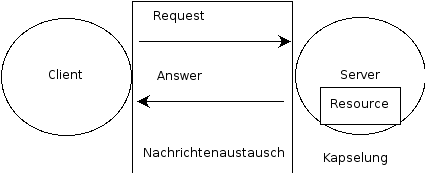
\includegraphics[width=100mm]{vs1.png}
\end{center}
\end{figure}
\subsubsection{Frage}
Gibt es in Java einen Adressraum?  Antwort: Ja (Siehe NullPointerException).\\
\\
Ein Prozess kann gleichzeitig Client und Server sein. 
\begin{figure}[htbp]
\begin{center}
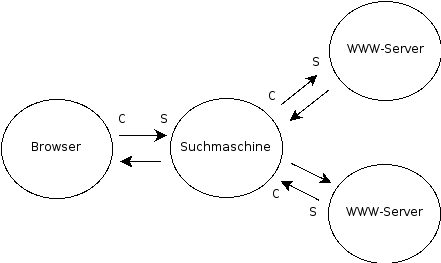
\includegraphics[width=105mm]{vs3.png}
\end{center}
\end{figure}
\"{A}hnliche Beziehung: Funktions- bzw. Methodenaufruf. Server werden ``st\"{a}ndig'' ausgef\"{u}hrt. Clients reden mit der \"{u}bergeordneten Applikation. Das Client-Server Modell beschreibt viele verteilte Systeme (nicht alle).

\section{Ziele beim Design eines verteilten Systems}

Ber\"{u}cksichtigt werden:

\begin{itemize}
	\item Heterogenit\"{a}t
	\item Offenheit
	\item Skalierbarkeit
	\item Sicherheit (gegen Angriffe)
	\item Fehlertoleranz
	\item Nebenl\"{a}ufigkeit
	\item Transparenz
\end{itemize}
\subsection{Heterogenit\"{a}t}
Heterogenit\"{a}t in den Bereichen
\begin{itemize}
	\item Netzwerk
	\item Computerhardware
	\item Betriebssysteme
	\item Programmiersprachen
\end{itemize}
Wesentliches Hilfsmittel zur Implementation heterogener Systeme: Einf\"{u}hrung einer Middleware.
Middleware ist eine Softwareschicht, die eine Programmierabstraktion zur Verf\"{u}gung stellt, und die Heterogenit\"{a}t des darunterliegenden Systems verbirgt.
\begin{figure}[htbp]
\begin{center}
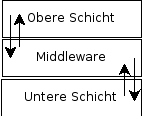
\includegraphics[width=30mm]{vs4.png}
\end{center}
\end{figure}
\\
Beispiele: Java, RMI, CORBA, SQL, RPC. (Bereitstellung einer einheitlichen Programmierschnittstelle).

\subsection{Offenheit}
Ziel Offenheit (Um sp\"{a}ter Erweiterungen vornehmen zu koennen). Z.B. Hinzuf\"{u}gung neuer Dienste f\"{u}r unterschiedliche Client-Programme.
\begin{itemize}
	\item Ziel wird erreicht durch Offenlegung der Spezifikation aller Softwareschnittstellen
	\item Wird unterst\"{u}tzt durch Standardisierung der Schnittstellen.
\end{itemize}
Beispiele f\"{u}r Offenheit:
\begin{itemize}
	\item Internet-Protokolle
	\item RFC (Request For Comment)\\
		\url{http://www.ietf.org}
\end{itemize}

\subsection{Skalierbarkeit}
Die Leistungsf\"{a}higkeit von Systemen soll durch Hinzuf\"{u}gen von Komponenten steigen. Steigender Bedarf an Dienstleistungen mu{\ss} mit beschr\"{a}nkten Kosten befriedigt werden.\\
\\
Ist ein Linux-Cluster ein skalierbares System? Nur schwer skalierbar (wg. Neuverkabelung bei Hinzunahme neuer Rechner).\\
\\
Wachstum bringt oft (relativen) Verlust an Leistung. Beispiel: Finden eines Objekts unter $n$ (Skalierungsgr\"{o}{\ss}e) Objekten. 

\begin{itemize}
	\item Bei linearem Suchen: Aufwand $\sim n$
	\item Bei bin\"{a}rem Suchen: Aufwand $\sim log(n)$
\end{itemize}
Angestrebt wird ein Aufwandswachstum $\approx log(n)$ ($n$ ``Gr\"{o}{\ss}e des Systems'').\\
\\
Weiteres Problem: Manche Ressourcen ersch\"{o}pfen sich! Beispiel: IP-Adressen. Leistungsengp\"{a}sse sollten durch Dezentralisierung vermieden werden!\\
\\
Anfangs: Ein zentraler DNS-Server, der ``alles'' in einer Datei wusste.

\subsection{Behandlung von Fehlern}

Erkennen von Fehlern: 

\begin{itemize}
	\item Pr\"{u}fsummen (``leicht m\"{o}glich'')
	\item Absturz eines Servers schwer zu erkennen
\end{itemize}
Maskierung von Fehlern:
\begin{itemize}
	\item Mehrfaches \"{U}bertragen von Nachrichten
	\item Mehrfache Speicherung von Daten
\end{itemize}
Frage: Greifen diese Ma{\ss}nahmen garantiert? Nein. Absolute Garantien kann man nie erwarten. Im Normalfall kann man die Sicherheit jedoch ausreichend ``hochschrauben''.\\
\\
``Tolerieren von Fehlern'' ist eine weitere Vorgehensweise. 
\begin{itemize}
	\item Weiterleitung von Fehlern an den Benutzer (\"{u}bergeordnete Schicht). Beispiele:
		\begin{enumerate}
			\item Browser findet Seite nicht
			\item Java: Exception 
			\item C: Nichts (nur einen Crash)
		\end{enumerate}
	\item Oft kann die Schicht, die den Fehler feststellt, nicht entscheiden, wie weiter vorzugehen ist. 
\end{itemize}
Zur Maskierung von Fehlern verwendet man oft redundante Komponenten. Beispiele:
\begin{itemize}
	\item Mehrere Routen im Netzwerk
	\item DNS: Jede Tabelle auf mehreren Servern
	\item Replizierte Datenbanken (Techniken sp\"{a}ter im Detail)
\end{itemize}

\subsection{Nebenl\"{a}ufigkeit}
``Gleichzeitige'' Benutzung von einer Ressource durch mehrere Benutzer. Ohne Nebenl\"{a}ufigkeit h\"{a}tten wir die sequentielle Benutzung von Ressourcen.
$\ra$ Schlechter Durchsatz.
\begin{figure}[htbp]
\begin{center}
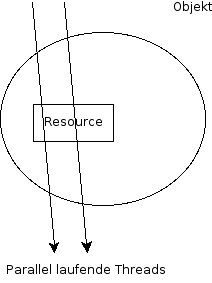
\includegraphics[width=33mm]{vs5.png}
\end{center}
\end{figure}
Im Allgemeinen lassen Server viele Clients gleichzeitig zu.  Ressource sei als Objekt gekapselt (Siehe Bild).\\
\\
In vielen F\"{a}llen ist die Synchronisation notwendig um inkonsistente Ergebnisse zu vermeiden. Objekte, die gemeinsam genutzte Ressourcen verwalten, m\"{u}ssen in einer nebenl\"{a}ufigen Umgebung \underline{korrekt} arbeiten.

\subsection{Transparenz}
Transparenz bedeutet, dass der Benutzer gewisse Details nicht ber\"{u}cksichtigen mu\ss, die die Implementation effizient machen.

\begin{itemize}
	\item \textbf{Zugriffstransparenz:} Lokale und entferne Zugriffe auf Objekte erfolgen mit den gleichen Methoden. Wenn man Sockets verwendet, kann man Nachrichten lokal und entfernt gleichartig verschicken.
	\item \textbf{Orts- und Positionstransparenz:} Man kann auf Ressourcen zugreifen, ohne ihren Ort zu kennen. Man kann die Ressourcen von verschiedensten Orten aus benutzen.
	\item \textbf{Nebenl\"{a}ufigkeitstransparenz:} Gemeinsame ``gleichzeitige'' Nutzung ohne Beeintr\"{a}chtigung. 
	\item \textbf{Replikationstransparenz:} Man arbeitet mit Repliken (Kopien) ohne Beeintr\"{a}chtigung.
	\item \textbf{Fehlertransparenz:} Partielle (teilweise) Ausf\"{a}lle beeintr\"{a}chtigen den Benutzer nicht.
	\item \textbf{Leistungs- und Skalierungstransparenz:} Das System kann neu konfiguriert oder erweitert werden, um h\"{o}here Leistungen zu erzielen.
\end{itemize}

\section{Systemmodelle}
Modelle heben strukturierte Eigenschaften von Systemen hervor und erm\"{o}glichen eine einheitliche Sichtweise auf verschiedenartige Realisationen.

\begin{itemize}
	\item \textbf{Architektonisches Modell:} Platzierung von Komponenten. Verbindungen und Beziehungen zwischen Komponenten.
	\item \textbf{Interaktionsmodell:} Zusammenspiel zwischen Teilen beim Nachrichtentausch.
	\item \textbf{Fehlermodell:} Beschreibung von Fehlerm\"{o}glichkeiten der Prozesse und Kommunikationskan\"{a}le. Festlegung was man als ``korrekt'' bzw. ``zuverl\"{a}ssig'' interpretiert.
	\item \textbf{Sicherheitsmodell:} Beschreibung von Gefahren durch Angriffe und Abwehrma{\ss}nahmen.
\end{itemize}
\subsection{Beispiele f\"{u}r architektonische Modelle}
\begin{itemize}
	\item Client - Server
	\item Peer to Peer (gleichrangige Prozesse)
	\item Schichten-Architektur 
\end{itemize}
\begin{figure}[htbp]
\begin{center}
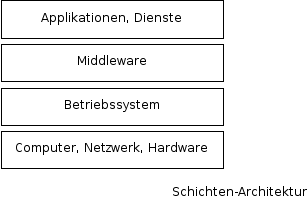
\includegraphics[width=60mm]{vs6.png}
\end{center}
\end{figure}
Die Middleware stellt zur Verf\"{u}gung:
\begin{itemize}
	\item Entfernte Methodenaufrufe
	\item Kommunikation in Gruppen
	\item Benachrichtigung \"{u}ber Ereignisse 
	\item Replikation von Daten
	\item Namensdienste (z.B. Matr.-Nr. in einer HS)
	\item Sicherheitskonzepte
	\item Transaktionen 
\end{itemize}
Die \"{U}bertragung von Aufgaben an die Middleware vereinfacht den Entwurf und die Implementation von verteilten Systemen.\\
\\
Aber es gibt Funktionalit\"{a}ten, die vollst\"{a}ndig und zuverl\"{a}ssig nur bei Kenntnis der Applikation implementiert werden k\"{o}nnen. Solche Funktionen kann man nicht vollst\"{a}ndig in Middleware verstecken.\\
\\
\textbf{Beispiel:} Ist TCP/IP die geeigente Middleware um Sicherheit beim Transport von E-Mails zu gew\"{a}hrleisten?\\
\\
$\ra$ TCP/IP ist daf\"{u}r nicht geeignet, weil z.B. keine geeigneten Ma{\ss}nahmen gibt, um l\"{a}ngere Ausf\"{a}lle von Servern zu maskieren!

\section{Interaktionsmodelle}
\begin{itemize}
	\item Wer kommuniziert mit wem, wann, warum, ... ?
	\item Wie beeinflusst das Timing von Nachrichten die Kommunikation und den Ablauf?
	\item Was ist der ``Zustand'' von einem verteilten Algorithmus?
\end{itemize}

\subsection{Synchrones verteiltes System}
\begin{itemize}
	\item F\"{u}r die Ausf\"{u}hrungszeit zu jedem Schritt eines Prozesses gibt es bekannte obere und untere Schranken.
	\item Jede Nachricht wird innerhalb einer begrenzten Zeit (fehlerfrei) empfangen.
	\item Die Abweichungsgeschwindigkeit von lokalen Uhren im Bezug wahren Zeit ist beschr\"{a}nkt. (\textit{Uhren gehen eigentlich nie zu 100 Prozent gleich. Die Abweichungsgeschwindigkeit ist das, wie schnell Uhren ``auseinanderwandern''})
\end{itemize}
Das sind sehr harte Forderungen! Von normalen Systemen sind diese nicht zu erf\"{u}llen. \textit{Dieses Modell ist eigentlich ein Wunschmodell.} (Wahrscheinliche Werte, Mittelwerte usw. sind oft leicht zu erf\"{u}llen).

\subsection{Asynchrones verteiltes System}
\begin{itemize}
	\item Keine Begrenzung f\"{u}r Prozessausf\"{u}hrung
	\item Unbegrenzte Nachrichtenverz\"{o}gerung
	\item Uhrabweichungen
\end{itemize}
Schon das ``Einigungsproblem'' zwischen 2 Teilnehmern im asynchronen System ist nicht l\"{o}sbar.

\section{Zeit und globale Zust\"{a}nde}
F\"{u}r Ereignisse gilt:
\begin{itemize}
	\item Man will wissen, ob ein Ereignis vor oder nach einem anderen Ereignis stattfand (\textit{Wir denken bisher mit vor und nach an die Zeit, sp\"{a}ter werden wir auch an was Anderes denken}).
	\item Man will wissen, ob man alle Informationen hat, die zu einem bestimmten Ereignis gef\"{u}hrt haben.
	\item Man will wissen, ob ein System (aus mehreren Komponenten) sich (zu einem Zeitpunkt) in einem Zustand befunden hat.
\end{itemize}
\textbf{Ansatz 1:} Versuche Uhren zu bauen\\
\\
\q $N$ Prozesse (evtl. auf verschiedenen Rechnern)\\
\\
\q Die echte wahre Zeit sei $t$.\\
\\
\q Hardwareuhr: $H_i(t) \quad i = 1, ..., N$\\
\\
\q Softwareuhr: $C_i(t) = \alpha * H_i(t) + \beta$\\
\\
Ziele: 
\begin{enumerate}
	\item $C_i(t) \approx t$\\
	\\
	$C_i(t) - t$ hei{\ss}t Uhrabweichung von Uhr $i$ zum Zeitpunkt $t$.
	\item $C_i(t) \approx C_j(t)$\\
	\\
	$C_i(t) - C_j(t)$ hei{\ss}t Synchronisationsfehler zwischen den Uhren $i$ und $j$ zum Zeitpunkt $t$.
\end{enumerate}
Uhren werden ``synchronisiert''. $S(t)$ sei eine Referenzuhr (z.B. UTC).
\begin{figure}[htbp]
\begin{center}
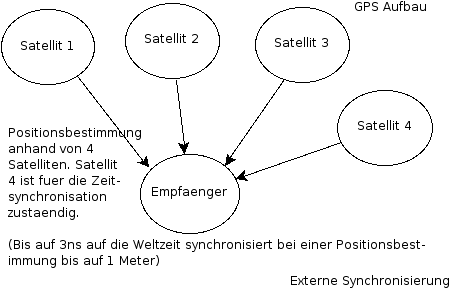
\includegraphics[width=115mm]{gps.png}
\end{center}
\end{figure}

\begin{enumerate}
	\item \underline{Externe Synchronisierung} \"{u}ber einem Zeitintervall gilt f\"{u}r alle $t \in I$:\\
\\
\q $|S(t) - C_i(t) | < D$ f\"{u}r alle $i = 1, ..., N$\\
\\
So heissen die Uhren $C_i$ mit $i = 1, ..., N$ extern synchronisiert mit Genauigkeit $D$. ($D$ ist fest f\"{u}r alle $i$, $t$). Uhrabweichung in $I$ ist kleiner als $D$.\\
\\
$5$ Sekunden Abweichungen pro Tag: $\frac{5s}{24 * 3600s} = 57 * 10^{-6} = 57ppm$\\
\\\textit{Bei billigen Uhren die man im Laden bekommt kann man leicht $10ppm$ erreichen. Atomuhren liegen bei einem Faktor von ca. $10^{-15}$.}
	\item \underline{Interne Synchronisierung} git f\"{u}r alle $t \in I$ und $i,j \in {1, ..., N}$ dass\\
	\\
	\q $|C_i(t) - C_j(t) | < D$\\
	\\
	so heissen die Uhren intern synchronisiert mit Genauigkeit $D$. (Uhren stimmen untereiander bis auf $D$ \"{u}berein.
\end{enumerate}
Ist ein System extern $D$-Synchronisiert, ist es intern garantiert $2D$-synchronisiert. Wenn ein System intern $D$-Synchronisiert ist, kann das zugeh\"{o}rige externe $D$ beliebig gro{\ss} sein.

\subsection{Einige Korrektheitsbegriffe f\"{u}r Uhren}

\textit{Eine Uhr die still steht, geht 2 mal am Tag richtig. Eine Uhr die 1 Minute vor geht, geht immer falsch?!? Es ist nicht einfach die Korrektheit einer Uhr zu definieren.}
\
\begin{enumerate}
	\item Eine Hardwareuhr hei{\ss}t korrekt, wenn ihre Abweichgeschwindigkeit (drift-rate) durch eine Schranke $\rho > 0$ begrenzt ist.\\
	\\
	D.h., der Fehler beim Messen von Intervallen zwischen Echtzeiten $t$ und $t'$ ist begrenzt durch:\\
	\\
	\q $(1-\rho) (t'-t) \le H(t') - H(t) \le (t'-t) (1+\rho)$\\
	\\
	\q $ \Leftrightarrow 1-\rho \le \frac{H(t')-H(t)}{t'-t} \le 1 + \rho$\\
	\\
	\q $ \ra -\rho \le \frac{H(t')-H(t)}{t'-t} -1 \le \rho$ (Gangabweichungsgeschwindigkeit)\\
	\\
	Erster Korrektheitsbegriff: Gangabweichungsgeschwindigkeit beschr\"{a}nkt.\\
	\\
	Frage: Darf eine in dem Sinne korrekte Uhr ``springen''? Antwort: \underline{nein}! \textit{Differenzierbare Funktionen m\"{u}ssen stetig sein}. Derartige Uhren d\"{u}rfte man nicht synchronisieren (``stellen''). $\ra$ Dieser Korrektheitsbegriff ist oft zu stark.
	
	\item Ein weiterer Korrektheitsbegriff: Eine Hardwareuhr hei{\ss}t korrekt, wenn sie ``monoton'' ist.\\
	\\
	\q $t < t' \ra H(t) < H(t')$\\
	\\
	$\ra$ Das ist oft ein zu schwacher Korrektheitsbegriff.

	\item Eine Hardwareuhr hei{\ss}t korrekt, wenn sie monoton ist und die Gangabweichung zwischen Synchronisationspunkten begrenzt ist. 
\end{enumerate}
\section{Methoden zur Synchronisation}
\subsection{Interne Synchronisation in einem synchronem System}
Annahme: Die Transportzeit einer Nachricht (vom Senden zum Empfangen) liegt garantiert zwischen $t_{min}$ und $t_{max}$. D.h. $t_{min} \le t_{tr} \le t_{max}$. Die anderen Zeiten seien vernachl\"{a}ssigibar. Nenne $t_{max} - t_{min}$ die ``Unsicherheit''.\\
\\
Prozess $P_1$ senden seine Zeit $t$ in einer Nachricht zu Prozess $P_2$.\\

\begin{figure}[htbp]
\begin{center}
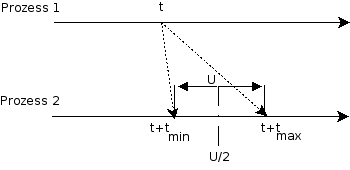
\includegraphics[width=85mm]{vs7.png}
\end{center}
\end{figure}
$P_2$ setzt beim Empfang seine Zeit auf:\\
\\
\q $t_2 = t + \frac{1}{2}(t_{max} + t_{min}) \ra$ Synchronisationsfehler $< \frac{U}{2}$\\
\\
Wenn man so $N$ Uhren intern synchronisiert, ist der Fehler $\le U(1-\frac{1}{N})$\\
\\
In asynchronen Systemen k\"{o}nnen keine Garantien gegeben werden.\\
\\
Beobachtung: Die Round-Trip Zeit (RTT) in realen Systemen ist oft relativ kurz.

\subsection{Christians Methode zur externen Synchronisation}
\begin{itemize}
	\item Es handelt sich um einen ``probabilistischen Algorithmus''.
	\item Mit Wahrscheinlichkeit $> p_0$ ist eine Synchronisation m\"{o}glich. 
	\item Typische Roundtrip-Zeiten sind $1, ..., 10ms$
	\item Abweichungsgeschwindigkeit der lokalen Uhr die zur Roundtrip-Zeimessung benutzt wird, ist vernachl\"{a}ssigbar klein.
	\item Der Prozess, der mit Round-Trip den Zeitserver nach der Zeit gefragt hat, setzt seine Zeit auf $t$ (Zeitpunkt des Servers) $ + \frac{T_{round}}{2}$ sofern man keine zus\"{a}tzlichen Informationen hat.
\end{itemize}
Christians Methode: Benutze die Round-Trip Zeit, um die Transportzeit von Nachrichten f\"{u}r den Einzelfall zu ``kennen''.\\
\\
Der Prozess p setzt seine eigene Zeit auf $t + \frac{T_{round}}{2}$. Mit $t :=$ Zeitstempel des Servers.
\begin{figure}[htbp]
\begin{center}
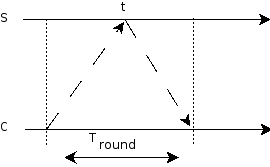
\includegraphics[width=70mm]{vs8.png}
\end{center}
\end{figure}
Annahme: Es ist etwas mehr bekannt, n\"{a}mlich eine untere Schranke $T_{min}$ f\"{u}r den Nachrichtentransport ($\ra T_{round} \le T_{min}$).
\begin{figure}[htbp]
\begin{center}
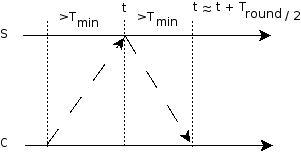
\includegraphics[width=75mm]{vs9.png}
\end{center}
\end{figure}
Client setzt seine Uhr wie vorher auf $t + \frac{T_{round}}{2}$. Die Genauigkeit ist $\pm(\frac{T_{round}}{2} - T_{min})$.\\
\\
Synchronisiere nur, wenn die beobachte Round-Trip-Zeit klein genug ist. Vorsicht: Beim Synchronisieren sind ggf. Korrektheitsbedinungen (Monotonie o.\"{A}...) zu beachten! 
\begin{itemize}
	\item Schutz gegen Ausfall: Einrichtung mehrerer Server.
	\item Erreichen kleinerer Round-Trip-Zeit: Benutze ``nahe'' Server.
	\item Problem: Betr\"{u}gerische Server: Kryptologische Methoden (Authentifizierung). \\
		Abgleich mehrerer Servern.
\end{itemize}

\subsection{Berkeley Algorithmus zur internen Synchronisierung}
\begin{itemize}
	\item Auswahll eines Koordinierungsmasters.
	\item Der Master fragt die Slaves ab. Diese senden ihre eigene Uhrzeiten zur\"{u}ck.
	\item Der Master sch\"{a}tzt die lokalen Zeiten der Slaves durch Beobachtung der Roundtrip-Zeit.
	\item Der Master bildet (durch gewichtete Mittelung) eine ``m\"{o}glichst genaue'' Referenzzeit.
	\item Der Master schickt allen Slaves ``Korrekturwerte'' die angeben, wie sie jeweils aus ihrer lokalen Zeit die Referenzzeit berechnen k\"{o}nnen.
\end{itemize}
Experiment: 15 Computer kann man in \"{u}blichen LANs relativ leicht auf ca. 25$\mu$s synchronisieren. (Bei ca 10ms Roundtrip)\\
\\
Keine Garantien!\\
\\
Problem (weiterhin): Uhren erm\"{o}glichen es nicht immer, die Frage zu beantworten, ob ein Ereignis a vor einem Ereignis b stattgefunden hat.\\
\\
Einf\"{u}hrung eines anderen Konzepts:
\section{Logische Zeit und logische Uhren}
Beobachtung: 
\begin{enumerate}
	\item Innerhalb eines Prozesses ist es leicht zu entscheiden, was ``fr\"{u}her'' oder ``sp\"{a}ter'' ist.
	\item Prozesse treten nur mit Nachrichten in Kontakt. (Keine Back-Channels)
\end{enumerate}
\textbf{Modellvorstellung:} Ein Prozess ist eine wohldefinierte Abfolge von Ereignissen.\\
\\
\textbf{Typische Ereignisse:} Senden einer Nachricht, Empfangen einer Nachricht, Berechnung eines Ergebnisses, \"{A}nderung eines Attributes eines Objekts, Speichern einer Datei. \\
\\
Idee (Lamport) definiere eine ``geschehen vor'' Relation. Relation zwischen zwei Ereignissen.\\

Schreibweise ``$\ra$''\\
\\
Zuerst f\"{u}r Ereignisse in einem Prozess $i$:\\
\\
$l_1 \ra_i l_2 \qquad l_1$ und $l_2$ im selben Prozess, dann ist die Reihenfolge klar.\\
\\
Die durch $\ra_i$ sortierte Folge der Ereignisse in einem Prozess nennt man eine ``history''. Klar ist: Eine Nachricht kann erst empfangen werden, nachdem sie gesendet wurde.\\
\\
Definiere die ``geschehen-vor'' Relation $\ra$ nun wie folgt:
\begin{enumerate}
	\item Falls es einen Prozess $i$ gibt, so dass\\
		$l \ra_i e'$ dann gillt $l \ra e'$
	\item F\"{u}r jede Nachricht $m$ gilt\\
		send($m$)$\ra$receive($m$)
	\item Es gilt $e\ra e'$ und $e'\ra e''$ dann gilt $e\ra e''\\$		
\end{enumerate}
Beispiel:
\newpage
\begin{figure}[htbp]
\begin{center}
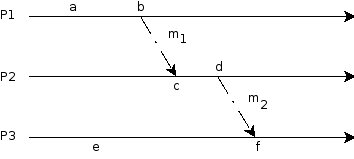
\includegraphics[width=90mm]{vs10.png}
\end{center}
\end{figure}

Ergibt:\\
\\
Wegen 1.: $\quad a\ra b \qquad c\ra d \qquad e\ra f$\\
Wegen 2.: $\quad b\ra c \qquad d\ra f$\\
\begin{figure}[htbp]
\begin{center}
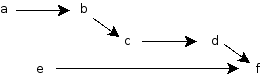
\includegraphics[width=60mm]{vs11.png}
\end{center}
\end{figure}
\\
Frage: Gilt $e\ra c$?? Kann es sein, dass f\"{u}r zwei Ereignisse $e$ und $e'$ sowohl $e\ra e'$ als auch $e'\ra e$ gilt? Antwort: Nein!
\begin{figure}[htbp]
\begin{center}
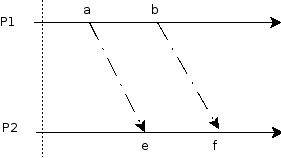
\includegraphics[width=70mm]{vs12.png}
\end{center}
\end{figure}
Hier gibt es zwei Begr\"{u}ndungen f\"{u}r $a\ra f$.\\
\\
Es gilt weder $a\ra e$ noch $e\ra a$ so bezeichnet man $a$ und $e$ als nebenl\"{a}ufig. Schreibweise: $a||e$\\
\\
Die ``geschehen vor'' Relation stellt einen m\"{o}glichen Datenfluss dar. Fragen der Art: ``Hat Ereignis $e_i$ das Ereignis $e_j$ m\"{o}glicherweise beeinflusst?'' sollen beantwortet werden.\\
\\
Wie stellt man ``$\ra$'' auf einem Rechner fest?\\
\\
Erster Ansatz:
\subsection{Logische Uhr von Lamport}
\begin{itemize}
	\item Jeder Prozess $i$ hat seine eigene logische Uhr $L_i$. $L_i$ w\"{a}chst monoton.
	\item Die eigene Zeit wird Nachrichten als Zeitstempel mitgegeben.
\end{itemize}
Wie wird $L_i$ jeweils aktualisiert? $L_i$ wird vor (bei) einem Ereignis in $P_i$ erh\"{o}t. 

\begin{itemize}
	\item Sendet Prozess $P_i$ eine Nachricht $m$, so wird der Nachricht der Zeitstempel $t=L_i$ mitgegeben.
	\item Beim Empfang einer Nachricht berechnet Prozess $P_j$ das Wort $L_j = max(L_j, t)+1$ und weist diesen Stempel dem Empfangsereignis zu.
	\item Die $L_i$ (Lamport-Zeitstempel) werden mit $0$ initialisiert.
\end{itemize}
\textit{Diese Definition wurde W\"{o}rtlich aus dem Buch abgeschrieben, nicht ganz Widerspruchsfrei. Daher wirds im Folgenden nochmal Veranschaulicht dargestellt}.\\
\begin{figure}[htbp]
\begin{center}
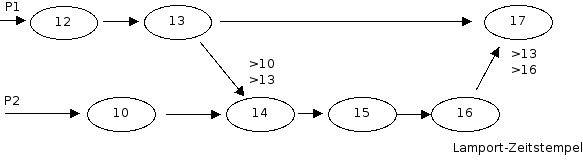
\includegraphics[width=110mm]{vs13.png}
\end{center}
\end{figure}
\\
Anschaulich: Das Empfangsereignis bekommt einen Zeitstempel der sowohl h\"{o}her ist als der Stempel des Sendeereignis als auch der Zeitstempel, der im eigenem Prozess vor ihm liegt.\\
\\
Frage: Was kann man aus Lamport-Zeitstempeln ableiten? Beispiel:\\
\begin{figure}[htbp]
\begin{center}
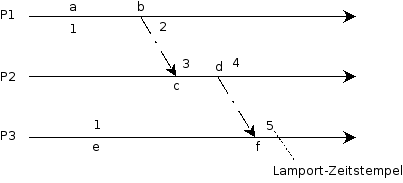
\includegraphics[width=100mm]{vs14.png}
\end{center}
\end{figure}
\begin{itemize}
	\item Wenn $e\ra e'$ dann gilt $L(e) < L(e')$
	\item Es gilt nicht: $L(e) < L(e') \Ra e\ra e'$ (Ein Beispiel: $L(b) > L(e)$ aber $e||b$)
	\item Man kann aus $L(e) < L(e')$ nur folgern $e' \not \rightarrow  e$
\end{itemize}
Manchmal gibt es Probleme, bei welchen sich alle Teilnehmer \"{u}ber eine Reihenfolge einig sein m\"{u}ssen, wobei egal ist, welche Reihenfolge es ist.\\
\\
\textbf{Beispiel:} Eine Bank f\"{u}hrt Konten mehrfach damit man gegen Abst\"{u}rze einzelner Server gesichert ist.
Transaktionen (\"{U}berweisungen) werden an alle Server geschickt.
F\"{u}r den Kunden ist die Ausf\"{u}hrungsreihenfolge von Transaktionen egal.\\
\\
Korrektheitsforderung: 
\begin{itemize}
	\item Jede einzele Transaktion mu{\ss} korrekt gesendet werden.
	\item Alle Server m\"{u}ssen zu dem gleichen Ergebnis kommen. D.h. die Server m\"{u}ssen sich auf eine (beliebige) Reihenfolge einigen.
\end{itemize}
Wenn die Server sich nicht einigen k\"{o}nnte folgendes passieren:
\begin{figure}[htbp]
\begin{center}
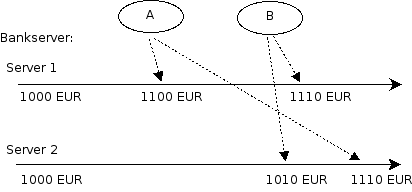
\includegraphics[width=100mm]{vs15.png}
\end{center}
\end{figure}
\begin{itemize}
	\item Kunde hat 1000 EUR
	\item Transaktion A: Einzahlung 100 \officialeuro
	\item Transaktion B: Verzinsung um 1\%
\end{itemize}
Dieses Probem kann mit Lamport-Zeitstempeln gel\"{o}st werden, wie im Folgendem gezeigt wird:\\
\\
Grundidee der L\"{o}sung: Alle Server m\"{u}ssen die Transaktionen in der gleichen Reihenfolge ausf\"{u}hren. Angewandtes Konzept ist ein ``vollst\"{a}ndig geordneter Multicast'' (Totally Ordered Multicast).\\
\\
\begin{figure}[htbp]
\begin{center}
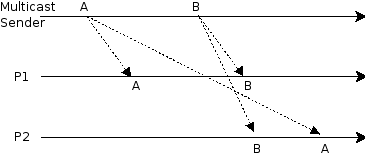
\includegraphics[width=90mm]{vs16.png}
\end{center}
\end{figure}
\begin{figure}[htbp]
\begin{center}
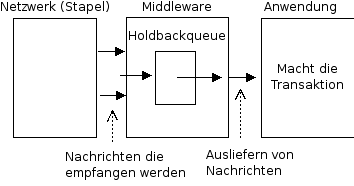
\includegraphics[width=90mm]{vs16b.png}
\end{center}
\end{figure}
Unterscheide von jetzt an konzeptionell zwischen dem Empfang von Nachrichten und der Auslierferung von Nachrichten. Bei einem ``vollst\"{a}ngig geordneten Multicast'' sorgt die Middleware daf\"{u}r, dass alle Anwendungen die Nachrichten in der gleichen Reihenfolge ausgeliefert bekommen.\\
\begin{enumerate}
	\item Teilschritt zur Realisation eines vollst. geordn. Multicasts mit Hilfe von Lamport Zeitstempeln: Erweitere die Lamport-Zeitstempel um die Rechner-Nummer (Prozess-ID o.\"{A}.) als Nachkommastelle!\\
	\\
	$\Ra$ Es gibt keine gleichen Zeitstempel mehr! D.h. f\"{u}r zwei verschiedene Ereignisse $e_1$ und $e_2$ gilt jetzt entweder $L(e_1) < L(e_2)$ oder $L(e_2) < L(e_1)$.
	\item Teilschritt: Implementiere damit den ``Totally Ordered Multicast'' wie folgt:\\
	\\
	Jede Nachricht bekommt den Zeitstempel des Senders und wird auch an den Absender gesandt. Empfangene Nachrichten werden in eine lokale Warteschlange eingef\"{u}gt die nach Zeitstempeln geordnet wird.\\
\begin{figure}[htbp]
\begin{center}
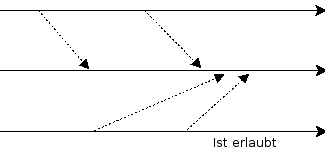
\includegraphics[width=70mm]{vs17.png}
\end{center}
\end{figure}
\\
Nun stelle eine weitere Forderung auf: Die Nachrichten die \underline{ein Sender} abschickt, kommen bei allen Empf\"{a}ngern in der Reihenfolge des Absendens an!
\begin{figure}[htbp]
\begin{center}
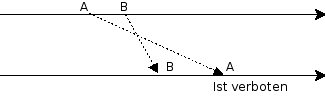
\includegraphics[width=70mm]{vs17b.png}
\end{center}
\end{figure}
Diese Forderung ist entscheidend, aber relativ leicht zu erf\"{u}llen (z.B. durch Nummerierung von Paketen oder verbindungsorientiertem Protokoll).\\
	\\
	Der Empf\"{a}nger einer Nachricht multicastet eine Best\"{a}tigungsnachricht (ACK Acknowledge) an alle anderen Prozesse. (Nachricht bekommt Zeitstempel und wird an den eigenen Absender gesandt!) Nun sammeln sich in den Warteschlangen die Originalnachrichten (die vollst. \textit{geordnet} ausgeliefert werden sollten) und die zugeh\"{o}rigen Best\"{a}tigungen.\\
	\\
	Eine Nachricht wird aus der Hold-Back Queue ausgeliefert, wenn sie an der Spitze steht und man von allen Prozessen die zugeh\"{o}rige ACK-Meldung bekommen hat.
\begin{figure}[htbp]
\begin{center}
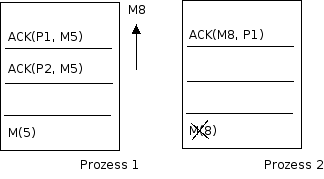
\includegraphics[width=70mm]{vs18.png}
\end{center}
\end{figure}
Damit werden Nachrichten erst ausgeliefert, wenn klar ist, dass alle anderen Prozesse diese Nachricht auch empfangen haben.\\
Vorsicht: Jede Nachricht die ``gemulticastet'' werden soll hat bei $N$ Teilnehmern $N^2$ ACK-Nachrichten zur Folge.
\end{enumerate}
Die Lamport-Zeitstempel waren nicht geeignet, die ``$\ra$''-Relation auf einfache Weise zu \"{u}berpr\"{u}fen. Deswegen: Erweiterung des Konzepts.

\subsection{Vektor-Zeitstempel}
\begin{itemize}
	\item $N$-Prozesse, jeder Prozess $I$ f\"{u}hrt seine eigene Vektor-Uhr $V_i$. Jede Vektor-Uhr $V_i$ ist ein Vektor mit $N$ Eintr\"{a}gen $V_i[j]$.
	\item Idee: $V_i[j] \quad$ (mit $i \ne j$) ist die Anzahl von Ereignissen in $P_j$, von welchen eventuell ein Datenfluss zu $P_i$ erfolgen konnte.
	\item $V_i[i]$ ist die Anzahl der Ereignisse, welchen $P_i$ selbst Zeitstempel zugewiesen hat.
	\item Initialisierung: $V_i[j] = 0 \quad$ f\"{u}r alle $i, j = 1 ..N$.
\end{itemize}
\begin{figure}[htbp]
\begin{center}
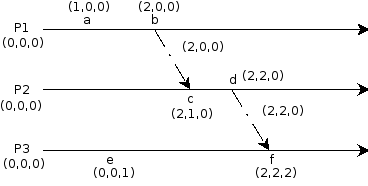
\includegraphics[width=85mm]{vs19.png}
\end{center}
\end{figure}
Zuweisung eines Zeitstempels zu einem Ereignis:
\begin{enumerate}
	\item Eigenzeit erh\"{o}hen $V_i[i] := V_i[i]+1$
	\item Bei einem Sendeereignis schickt man den eigenen Zeitstempel in der Nachricht mit, d.h. die korrekte Vektoruhr.
	\item Beim Empfang: Nach Erh\"{o}hen der Eigenzeit (vgl. 1) Bildung des Maximums aus empfangenem Zeitstempel und eigener Vektoruhr (elementweise) ergibt neue Vektoruhrzeit.
\end{enumerate}
\subsubsection{Vergleich von Vektorzeitstempeln}
\begin{itemize}
	\item $v=v' \quad$ iff $\quad v[j] = v'[j]\quad$ ist f\"{u}r alle $j$
	\item $v\le v' \quad$ iff $\quad v[j] \le v'[j]\quad$ ist f\"{u}r alle $j$
	\item $v< v' \quad$ iff $\quad v[j] \le v'[j]$ und $v\ne v'\quad$ ist f\"{u}r alle $j$
\end{itemize}
Man kann zeigen: $e\ra e' \Ra v(e) < v(e')$ \textit{Das ging auch schon bei Lamport-Zeitstempeln}. $\quad$ und $v(e)<v(e') \Ra e\ra e'$. \textit{Das ging bei den Lamport-Zeitstempeln noch nicht}.\\
\\
Man kann erkennen, ob Ereignisse nebenl\"{a}ufig sind: $x||y$ wenn weder $x\le y$ ist noch $y\le x$ ist.\\
\\
D.h. Vektorzeitstempel erlauben es, die ``$\ra$''-Relation auszuwerten. 
\textbf{Nachteil:} Hoher Aufwand (Speicher und Netzlast) bei gr\"{o}sserem $N$. \textbf{Aber:} Es gibt kein Verfahren mit ``kleinerem Aufwand'' um durch Vergleich logischer Uhren Nebenl\"{a}ufigkeit festzustellen.

\section{Globale Zust\"{a}nde}
\textbf{Aufgabe:} Man mu{\ss} feststellen k\"{o}nnen ob bestimmte Situationen vorliegen.\\
\\
\textbf{Beispiele:}
\begin{itemize}
	\item Ist ein Objekt \"{u}berfl\"{u}ssig? (Garbage Collection)
	\item Ist ein verteilter Algorithmus fertig?
	\item Ist ein Deadlock vorhanden?
	\item Ist garantiert, dass Ereignis $A$ ``vor'' Ereignis $B$ auftritt?
	\item Kann es m\"{o}glicherweise passieren, dass zwei Benutzer eine Datei gleichzeitig benutzen?
\end{itemize}
Zur verteilten Garbage Collection: 
\begin{figure}[htbp]
\begin{center}
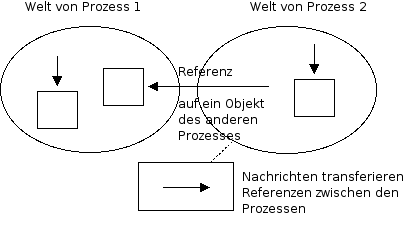
\includegraphics[width=105mm]{vs20.png}
\end{center}
\end{figure}
Objekte werden durch Referenzen benutzbar. Referenzen, die  momentan transferiert werden, m\"{u}ssen ber\"{u}cksichtig werden.\\
\\
Das Erkennen, ob ein Algorithmus in einem verteilten System abgeschlossen ist, kann z.B. schwer sein, wenn folgendes gemacht wird:\\
\\
Prozesse warten (passiv) auf Aktivierung (d.h. Zusendung eines Arbeitspaketes).
\begin{figure}[htbp]
\begin{center}
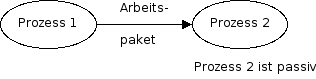
\includegraphics[width=85mm]{vs21.png}
\end{center}
\end{figure}
W\"{a}hrend das Paket unterwegs ist, sind alle Prozesse ``passiv'', aber der Algorithmus noch nicht abgeschlossen.\\
\\
Problem: Weil es keine globale Zeit gibt, ist man nicht in der Lage eine Momentaufnahme (Snapshot) des Systems herzustellen. Deswegen kann man nicht feststellen ob zu einer Zeit $t$ eine Situation vorliegt.\\
\\
\textbf{Frage:} kann man aus lokalen Zust\"{a}nden, die zu unterschiedlichen Zeiten aufgenommen wurden, einen sinnvollen globalen Zustand zusammensetzen?\\
\\
\textit{Einfache aber schlechte} \textbf{Antwort:} Manchmal.\\
\\
Antworten auf Fragen der Art: 
\begin{itemize}
	\item H\"{a}tte das System in dem Zustand $X$ sein k\"{o}nnen?
	\item Ist das System garantiert nie im Zustand $X$ gewesen?
\end{itemize}
sind teilweise m\"{o}glich.
\newpage
\subsection{Konzepte zur ``Formalisierung''}
\subsubsection{Idee des ``Schnittes'' eines Systems}
\begin{figure}[htbp]
\begin{center}
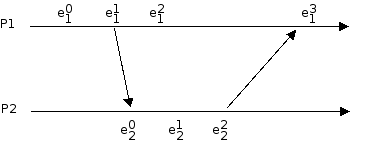
\includegraphics[width=95mm]{vs22.png}
\end{center}
\end{figure}
~\\
Die ``History'' von $P_1$ ist $e_1^0\quad e_1^1\quad e_1^2\quad e_1^3\quad ...$\\
\\
Die ``History'' von $P_2$ ist $e_2^0\quad e_2^1\quad e_2^2\quad e_2^3\quad ...$\\
\\
\begin{tabular}{cccc|}
$e_1^0$ & $ e_1^1$ & $ ... $ & $ e_1^k$\\
$e_2^0$ & $ e_2^1$ & $ ... $ & $ e_2^j$
\end{tabular}
\\
\\
\textit{$e_1^k$ und $e_2^j$ bilden die Front eines Schnittes. Die Front einschliesslich alle vorherigen Zust\"{a}nde sind ``im Schnitt enthalten''}\\
\\
Ein m\"{o}glicher Schnitt des obigen Systems w\"{a}re:\\
\\
\begin{tabular}{ccc|}
~ & ~ & $e_1^0$\\
$e_2^0$  & $e_2^1$ & $e_2^2$
\end{tabular}
\\
\\
\\
Ein Schnitt ist konsistent, wenn f\"{u}r jedes Ereignis des in ihm enthalten ist, auch alle Ereignisse enthalten sind, die im Sinne der ``geschehen vor''-Relation ``vor ihm'' liegen.\\
\\
Der Schnitt \textit{von oben} ist inkonsistent, weil z.B. $e_1^1 \ra e_2^0$ und $e_2^0$ ist im Schnitt und $e_1^1$ ist nicht im Schnitt.
\begin{figure}[htbp]
\begin{center}
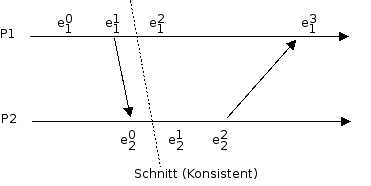
\includegraphics[width=95mm]{vs23.png}
\end{center}
\end{figure}
Ein konsistenter globaler Zustand wird definiert als konsistenter Schnitt. Der Zustand eines Systems entspricht nie einen inkonsistenten Schnitt.\\
\\
Die konsistenten Schnitte ensprechen alle m\"{o}glichen Situationen. Ein verteiltes System bewergt sich durch konsistente globale Zust\"{a}nde.\\

$S_0 \ra S_1 \ra S_2 \ra ...$\\
\\
Ereignisse ``$\ra$'' in einzelnen Prozessen: ``Senden'', ``Empfangen'', ``inneres Ereignis''.\\
\\
Ein ``RUN'' ist eine Anordnung aller Ereignisse in einem System die konsistent ist mit jeder lokalen history. F\"{u}r das obige System ist\\

$e_1^0 \quad e_1^1 \quad e_1^2 \quad e_1^3 \quad  e_2^0 \quad  e_2^1 \quad e_2^2$\\
\\
ein RUN.\\
\\
Ist ein RUN auch konsistent mit der globalen ``geschehen vor''-Relation, nennt man ihn eine Linearisierung des Systems. Es kann mehrere Linearisierungen geben! 
\begin{figure}[htbp]
\begin{center}
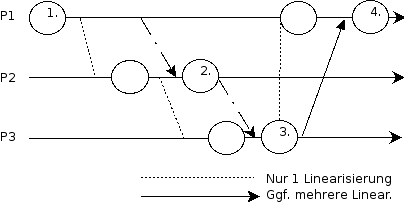
\includegraphics[width=100mm]{vs24.png}
\end{center}
\end{figure}
\subsection{Auswertung von Pr\"{a}dikaten in globalen Zust\"{a}nden}
Interessante Pr\"{a}dikate:
\begin{itemize}
	\item System ist in einem Deadlock
	\item Objekt ist ``Garbage''
	\item Prozess ist terminiert
	\item Ein Attribut eines Objektes hat einen bestimmten Wert
\end{itemize}
F\"{u}r viele Pr\"{a}dikate ist die Auswertung schwer. Deswegen definiert man ``neue Pr\"{a}dikate'' mit Hilfe der gew\"{u}nschten Pr\"{a}dikate.\\
\\
$\varphi$ ist ein Pr\"{a}dikat das in einem globalen Zustand ausgewertet werden kann.\\
\\
M\"{o}glicherweise $\varphi \quad$ iff $\quad$ Es gibt einen konsistenten globalen Zustand $S$, der eine Linearisierung der Hostorie $H$ durchl\"{a}uft, so dass $\varphi(S) = true$. 
\begin{figure}[htbp]
\begin{center}
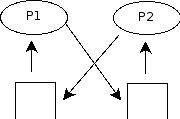
\includegraphics[width=40mm]{vs25.png}
\end{center}
\end{figure}
\begin{figure}[htbp]
\begin{center}
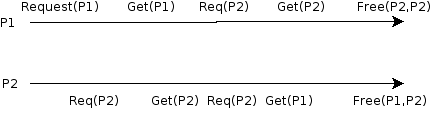
\includegraphics[width=100mm]{vs25b.png}
\end{center}
\end{figure}
Definitiv $\varphi \quad$ iff $\quad$ F\"{u}r alle Linearisierungen $L$ von $H$ gibt es einen konsistenten globalen Zustand $S$ (der kann von der Linearisierung abh\"{a}ngen) den $L$ durchl\"{a}uft mit $\varphi(S) = true$.\\
\\
Vorsicht: $\overline{moeglicherweise} \quad \varphi \ra definitiv \quad \overline{\varphi}$\\
\\
aber\\
\\
aus definitiv $\overline{\varphi}$ $\not{\ra}$ $\overline{moeglicherweise \quad \varphi}$\\ 
\\
Oft interessieren einen ``stabile Pr\"{a}dikate''. Ein Pr\"{a}dikat hei{\ss}t stabil, wenn daraus, dass es einen Zustand wahr ist folgt, dass es in m\"{o}glichen Folgezust\"{a}nde wahr ist.\\
\\
Anschaulich:\\
\\
M\"{o}glicherweise $\varphi$:$\quad$M\"{o}glicherweise hat sich das System so entwickelt, dass zu irgendeinem Zeitpunkt einmal $\varphi$ galt.\\
\\
Definitiv $\varphi$:$\quad$Das System hat sich definitiv so entwickelt, dass auf jeden Fall in irgendeinem Zustand $\varphi$ galt.\\
\\
\textbf{Beispiel:} 
\begin{itemize}
	\item Objekte k\"{o}nnen von Prozessen ``gelockt'' werden
	\item $L(x)$ Lock auf ein Objekt haben
	\item $U(x)$ Unlock (Lock sperrt) zur\"{u}ckgeben
\end{itemize}
Pr\"{a}dikat $\varphi$ ``es liegt ein Konflikt vor''. D.h. wenn ein Objekt zweimal gelockt wurde, liegt ein Konflikt vor. 
\begin{figure}[htbp]
\begin{center}
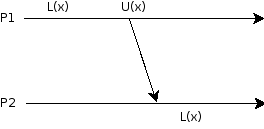
\includegraphics[width=70mm]{vs26.png}
\end{center}
\end{figure}
\begin{itemize}
	\item definitiv (Konflikt) nein
	\item m\"{o}glicherweise (Konflikt) nein
	\item definitiv (kein Konflikt) ja
	\item m\"{o}glicherweise (kein Konflikt) ja
\end{itemize}
\newpage
\begin{figure}[htbp]
\begin{center}
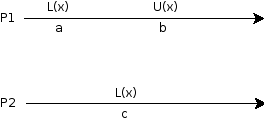
\includegraphics[width=70mm]{vs27.png}
\end{center}
\end{figure}
Alle Linearisierungen des Systems: $abc$, $acb$, $cab$.
\begin{itemize}
	\item definitiv (Konflikt) nein $abc$
	\item m\"{o}glicherweise (Konflikt) ja $acb$
	\item definitiv (kein Konflikt) ja am Anfang
	\item m\"{o}glicherweise (kein Konflikt) ja am Anfang
\end{itemize}
\begin{figure}[htbp]
\begin{center}
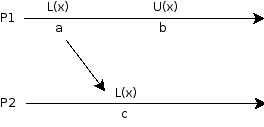
\includegraphics[width=70mm]{vs28.png}
\end{center}
\end{figure}
Reicht noch nicht um ``definitiv (Konflikt)'' wahr zu machen (denn es gibt noch die Linearisierung $abc$ die konfliktfrei ist)
\begin{figure}[htbp]
\begin{center}
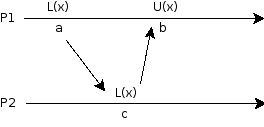
\includegraphics[width=70mm]{vs29.png}
\end{center}
\end{figure}
\begin{itemize}
	\item definitiv (Konflikt) ja
	\item m\"{o}glicherweise (Konflikt) ja
	\item definitiv (kein Konflikt) nein
	\item m\"{o}glicherweise (kein Konflikt) nein
\end{itemize}

\section{Koordination und \"{U}bereinstimmung}
Grundprobleme:
\begin{itemize}
	\item Zugriff auf gemeinsam genutzte Ressourcen mu{\ss} koordiniert werden.
	\item In vielen Situationen mu{\ss} Einigkeit hergestellt werden (z.B. wer der Master ist, ob eine Transaktion g\"{u}ltig ist, ...).	
\end{itemize}
Algorithmmus f\"{u}r wechselseitigen Ausschluss:\\
\\
$N$ Prozesse $P_i\quad i = 1 ... N \quad$ greifen mit dem folgenden Protokoll auf eine Ressource zu:
\begin{itemize}
	\item enter(): Eintritt in den kritischen Bereich (ggf. blockiert)
	\item exit(): Kritischen Bereich verlassen
\end{itemize}
Anforderungen an einem Algorithmus zur Realisierung des wechselseitigen Ausschlusses:
\begin{enumerate}
	\item Sicherheit: H\"{o}chstens ein Prozess ist zu einer Zeit in einem kritischen Bereich.
	\item Liveness: Anforderungen in dem kritischen Bereich einzutreten sind irgendwann erfolgreich.
	\item Reihenfolgeforderungen: Reihenfolge des Eintretens darf nicht gegen die ``$\ra$''-Relation zwischen Anforderungen verstossen. \textit{Diese Anforderung ist schwer zu erf\"{u}llen, daher wird diese vorerst weggelassen}.
\end{enumerate}
Bewertung und Messung der Leistungsf\"{a}higkeit von Algorithmen in verteilten Systemen:
\begin{itemize}
	\item ``Verbrauchte Bandbreite'' (Anzahl der Nachrichten pro enter/exit-Operationen)
	\item ``Client-Verz\"{o}gerung'' bei jeder enter/exit-Operation. 
	\item ``Systemdurchsatz'': Wieviele Vorg\"{a}nge erreicht man pro Zeiteinheit.
\end{itemize}

\subsubsection{Beispiel 1} 
...f\"{u}r ein Verfahren zur Sicherung des ``wechselseitigen Ausschlusses''.\\
\\
Algorithmus mit zentralem ``Token''-Server. Ein Zentralserver vergibt \underline{``ein Token''} an einen Client, der Zugriff auf die Ressource haben will. Der Client, der das Token besitzt, darf die Ressource benutzen. Nach der Benutzung gibt der Client das Token an den Zentralserver zur\"{u}ck.
\begin{itemize}
	\item Annahme: Der Nachrichtenaustausch ist fehlerfrei. Wechselseitiger Ausschluss wird durch die Einmaligkeit des Tokens gew\"{a}hrleistet.
	\item Sortiere die eingehenden Anfragen nach Tokens in FIFO-Ordnung. Dann bekommt jeder Prozess der anfragt irgendwann den Zugriff weil in der Warteschlange nur endlich viele Prozesse vor ihm stehen und jeder von diesen das Token nach Benutzung der Ressource zur\"{u}ckgibt.
	\item Dabei gehen wir davon aus, dass Prozesse nie abst\"{u}rzen.
	\item Aufwand zum Eintritt in den kritischen Bereich: $2$ Nachrichten f\"{u}r den Eintritt (Anfrage und \"{U}bermittlung des Tokens).
	\item Beim Verlassen: Eine Nachricht: R\"{u}ckgabe des Tokens.
	\item Wenn der Eintritt unmittelbar erfolgreich ist, dauert das nur eine Round-Trip Zeit.
	\item Nachteil des Verfahrens ist die starke Abh\"{a}ngigkeit vom Zentralserver der eventuell durch viele Anfragen \"{u}berlastet wird.
\end{itemize}
Alternative ohne zentralen Server: Token-Ring
\begin{itemize}
	\item Jeder Teilnehmer, der das Token besitzt, aber nicht ben\"{o}tigt, schickt es weiter. Das Token wird von allen ``in die gleiche Richtung'' weitergeschickt, damit jeder das Token irgendwann erh\"{a}lt.
	\item Vorsicht: Nachteil ist, dass st\"{a}ndig Nachrichten versandt werden, auch wenn niemand in den kritischen Bereich will.
	\item Verz\"{o}gerung: Im schlimmsten Fall sind bei $N$ Teilnehmern $N$ Nachrichtenzeiten notwendig.
	\item Man k\"{o}nnte (z.B. mit einem Multicast) alle Teilnehmer ``gleichzeitig'' nach dem Token fragen. Im erfolgreichen Fall ist das schnell!
	\item Ausbauen der Idee $\Ra$ Verfahren von Ricart - Agruala\\
		\\
		Das Verfahren ist relativ schnell und es lassen sich zus\"{a}tzlich Reihnfolgengarantien erbringen, aber man braucht \underline{Multicasts}. $\Ra$ Hohes Nachrichtenaufkommen
	\item Anderes Konzept: Wahl-Algorithmus von Maekawa. Idee:
		\begin{enumerate}
			\item Jeder Prozess $P_i$ erh\"{a}lt eine W\"{a}hlermenge $V_i$ und zwar, wenn alle in $V_i$ enthaltenen Prozesse zustimmen, bekommt $P_i$ das Zutrittsrecht.
			\item Jeder Prozess darf nur eine Stimme abgeben.
		\end{enumerate}
		Wie sehen die W\"{a}hlermengen aus:\\
		\\
		$V_i = \{ P_1, ..., P_N \}$\\
		\\
		Und f\"{u}r alle $i, j = 1... N$ gilt:
		\begin{enumerate}
			\item $P_i \in V_i$
			\item $V_j \cap V_i \ne \{ \}$ Je zwei W\"{a}hlermengen enthalten mindestens ein gemeinsames Element!!!
			\item $|V_i| \approx k$ d.h. alle W\"{a}hlermengen haben (ungef\"{a}hr) die gleiche Gr\"{o}sse ``F\"{a}irness''
			\item Jeder Prozess $P_j$ ist in $M$ der W\"{a}hlermengen enthalten. ``Gleich-Wichtigkeit\\ aller Prozesse.
		\end{enumerate}
		Frage: Warum ist wechselseitiger Ausschluss gesichert?\\
		\\
		Annahme: Zwei Prozesse $P_a$ und $P_b$ haben beide das Zugriffsrecht erhalten.\\
		\\
		$\Ra$ $P_a$ und $P_b$  haben die jeweils notwendigen Stimmen aus $V_a$ und $V_b$ erhalten.\\
		\\
		$\Ra$ (Wegen 2) ein Prozess (der in $V_a$ und $V_b$ enthalten ist) hat $2$ Stimmen abgegeben $\Ra$ Widerspruch\textit{, wechselseitiger Ausschluss ist gesichert}.\\
		\\
		Maekawa: Es gilt $k\approx\sqrt{N}\quad k\approx M$\\
		\\
		Berechnung der optimalen W\"{a}hlermengen ist sehr schwer!\\
		\\
		Es geht einfach: $|V_i|\approx 2\sqrt{N}$\\
		\\
		Annahme $N$ ist eine Quadratzahl z.B. $N=9$.\\
		\\
		\begin{tabular}{ccc}
		1 & 2 & 3 \\
		4 & 5 & 6 \\
		7 & 8 & 9 
		\end{tabular}
		\\
		\\
		$V_1 = \{1, 2, 3, 4, 7\}$\\
		$V_2 = \{1, 2, 3, 5, 8\}$\\
		$V_3 = \{1, 2, 3, 6, 9\}$\\
		$V_4 = \{1, 4, 5, 6, 7\}$\\
		$V_5 = \{2, 4, 5, 6, 8\}$\\
		$V_6 = \{3, 4, 5, 6, 9\}$\\
		$V_7 = \{1, 4, 7, 8, 9\}$\\
		$V_8 = \{2, 5, 7, 8, 9\}$\\
		$V_9 = \{3, 6, 7, 8, 9\}$\\
		\\
		Jede W\"{a}hlermenge enth\"{a}lt $2n-1$ Elemente $= 2\sqrt{N}-1$ Elemente.\\
		\\
		Jedes Element ist in $2n-1$ W\"{a}hlermengen enthalten.\\
		\\
		Durch die Konstruktion ist sichergestellt, dass zwei beliebige W\"{a}hlermengen mindestens 1 gemeinsames Element haben (Schnittpunkte von Zeilen oder Spalten).\\
		\\
		Der Algorithmus mu{\ss} noch ``Deadlock-frei'' gemacht werden, damit er wirklich anwendbar ist, das geht!\\
		\\
		Weil die W\"{a}hlermengen im Vergleich zu $N$ (Teilnehmerzahl) klein sind, ist das Verfahren relativ schnell. Nachrichtenaufwand $2\sqrt{N}$ (falls $k=M=\sqrt{N}$) n\"{a}mlicn $\sqrt{N}$ mal Anfrage nach Zustimmung.\\
		\\
		Was f\"{u}r Fehler sind problemantisch:
		\begin{itemize}
			\item Verlust von Nachrichten wird nicht toleriert.
			\item Wenn einzelne Prozesse abst\"{u}rzen, sind nicht sofort alle betroffen. Manchmal entsteht durch einen Einzelausfall noch kein Gesamtausfall.
		\end{itemize}
		Modifikationen um Fehler zu entdecken und zu tolerieren sind oft m\"{o}glich. Dazu braucht man in einem verteilten System die M\"{o}glichkeit, Fehler zu entdecken.
\end{itemize}

\section{Fehlerdetektor}
Ein Fehlerdetektor ist ein Dienst, der Abfragen beantwortet ob ein bestimmter Prozess fehlgeschlagen bzw. abgest\"{u}rzt ist! Er liefert die Antwort unverd\"{a}chtig (unsuspected) oder verd\"{a}chtigt (suspected).\\
\\
Vergleiche Brandmelder:
\begin{itemize}
	\item Ein Prozess wird als verd\"{a}chtig eingestellt obwohl er korrekt arbeitet. Das darf ab und zu passieren. 
	\item Ein Prozess arbeitet nicht korrekt, wird er als unverd\"{a}chtig eingestuft. Das sollte nach M\"{o}glichkeit nicht passieren.
	\item Man kann ``Time-Outs'' verwenden, um Prozesse als ``fehlgeschlagen'' zu identifizieren.
\end{itemize}
Ein weiteres Koordinationsproblem: Wahl genau eines Prozesses. (z.B. um die Rolle eines Koordinators zu \"{u}bernehmen). Alle Prozesse sind gleichberechtigt.\\
\\
\"{U}blicher Ablauf:
\begin{enumerate}
	\item Ein Prozess (oder mehrere) initiiert eine Wahl (Grund k\"{o}nnte z.B. sein, dass ein Teilnehmer festgestellt hat, dass ein zentraler Server, der bisher Koordinator war, abgest\"{u}rzt ist.)
	\item Wahl selbst
	\item Verteilung des Wahlergebnisses
\end{enumerate}
Ziel: Fehlertoleranz gegen Absturz von Prozessen. Bei erfolgreicher Wahl: Einigkeit dar\"{u}ber, wer Koordinator ist. Einigkeit dar\"{u}ber, ob die Wahl erfolgreich war.

\subsection{Teilproblem}
Sichere Multicast-Kommunikation (\textit{Beim Verteilen eines Wahlergebnisses soll der Verteiler z.B. selbst nicht abst\"{u}rzen}). 
\begin{itemize}
	\item Anwendung: Gruppenkommunikation und Koordination.
	\item Ziel: \underline{Auslieferung}sgarantie. (\textit{Das ist keine Empfangsgarantie})
\end{itemize}
UDP/IP Multicasts erbringen \"{u}blicherweise keinerlei Garantie. Sie bieten aber oft die M\"{o}glichkeit, Nachrichten relativ schnell an relativ viele Empf\"{a}nger weiterzuleiten.\\
\\
Vorteil von Multicasts: Sendende Prozess macht nur eine Send-Operation, die als atomar gilt. Normalerweise kann man Multicasts effizienter realisieren als das Nacheinandersenden mit 1:1 Kommunikation.\\
\\
Nun versuche ein Verefahren f\"{u}r einen zuverl\"{a}ssigen Multicast anzugeben. 
\begin{itemize}
	\item Voraussetzung: Zu jedem Prozess hat jeder andere Prozess eine zuverl\"{a}ssige 1:1 Verbindung.
	\item Operationen: 
		\begin{itemize}
			\item \textbf{multicast($g$,$m$)} mit \\
				$g :=$ Gruppe in welcher der Multicast stattfindet \\
				$m :=$ Nachricht
			\item \textbf{deliver($m$)} Auslieferung einer Nachricht an einem empfangenden Prozess\\
				\\
				(Vorsicht: Auslieferung erfolgt nicht sofort beim Empfang sondern eventuell sp\"{a}ter, eventuell gar nicht.)
		\end{itemize}
		\item Ein Prozess multicasted auch an sich selbstm. D.h. die Multicast-Nachricht wird (im erfolgreichen Fall) auch an den Initiator des Multicasts ausgeliefert.
		\begin{figure}[htbp]
		\begin{center}
		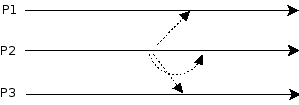
\includegraphics[width=75mm]{vs31.png}
		\end{center}
		\end{figure}
\end{itemize}
\subsubsection{Grundlegender (Basic Multicast)} wird wie folgt implementiert:\\
\\
$~\quad$ B-multicast($g$,$m$):\\
$~\qquad$ f\"{u}r jeden Prozess $p \in g$\\
\\
$~\quad$ Bei receive($m$) in $p~$:\\
$~\qquad$ B-deliver($m$) in $p$\\
\\
Problem: Es kann sein, dass der Sender abst\"{u}rzt nachdem einige Send-Operationen schon durchgef\"{u}hrt wurden, und einige noch nicht. Deswegen ist der Basic-Multicast kein zuverl\"{a}ssiger Multicast. Es ist nicht sichergestellt, dass alle Teilnehmer in der Gruppe entweder $m$ ausliefern, oder keiner.
\subsubsection{``Zuverl\"{a}ssiger Multicast\''} (\underline{R}eliable-Multicast).\\
\\
Voraussetzung: 
\begin{itemize}
	\item Integrit\"{a}t: Die ausgelieferte Nachricht ist gleich der Gesendeten. Keine Nachricht wird doppelt ausgeliefert.
	\item Liveness: Jede Nachricht erreicht ihr Zeil, sofern das Ziel \textit{bzw. der Zielprozess} nicht abgest\"{u}rzt ist.
	\item Einigung: Wenn \underline{ein} Prozess die Nachricht ausliefert, liefern alle korrekten Prozesse die Nachricht irgendwann aus (korrekt hei{\ss}t hier: Nicht abgest\"{u}rzt.).
	\item Einigungsbedingung: ``Alles oder Nichts'' (\textit{Hier besser formuliert: Alle oder Keiner})
	\item Fehlertoleranz: Einzelne Empf\"{a}nger oder Sender d\"{u}rfen abst\"{u}rzen.
\end{itemize}
\textit{Verfahren/Algorithmus siehe Aush\"{a}ndigung}
\begin{figure}[htbp]
\begin{center}
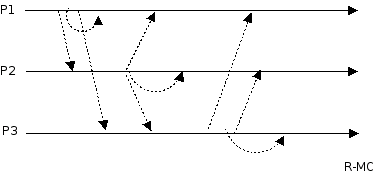
\includegraphics[width=75mm]{vs32.png}
\end{center}
\end{figure}
Jeder Prozess liefert erst dann aus, wenn er selbst den B-multicast erfoglreich hinter sich gebracht hat. Der B-Multicast verwendet sichere 1:1 Kan\"{a}le.
\begin{figure}[htbp]
\begin{center}
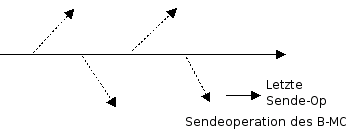
\includegraphics[width=75mm]{vs33.png}
\end{center}
\end{figure}
Wenn ein Prozess das Ende seines B-Multicasts erlebt, kann er sicher sein, dass alle Prozesse die noch weiterleben seine Nachricht noch bekommen haben und diese irgendwann ausliefern, sofern sie nicht vorher abst\"{u}rzen.\\
\\
Mit Hilfe eines verl\"{a}sslichen Multicasts lassen sich viele Koordinationsprobleme L\"{o}sen.\\
\\
Ein weiteres Beispielproblem: Herstellen von Konsens
\begin{itemize}
	\item Ein oder mehrere Prozesse schlagen Werte vor.
	\item Die Prozesse einigen sich auf einen dieser Werte.
	\item Konsens soll selbst dann erzielt werden, wenn Fehler vorkommen.
\end{itemize}
Folgendes Fehlermodell:
\begin{itemize}
	\item $f$ von $N$ Prozessen arbeiten fehlerhaft (Sind z.B. fehlerhaft programmiert oder betr\"{u}gen)
	\item Der Nachrichtenaustausch ist fehlerfrei. 
	\item Das System sei synchron.
\end{itemize}
F\"{u}r $N \ge 3 f + 1$ ist das Konsensproblem l\"{o}sbar! Man braucht mindestens $f+1$ Nachrichtenrunden.\\
\\
Ein Beispiel f\"{u}r ein ``unl\"{o}sbares Konsensproblem'':
\begin{itemize}
	\item Zwei (befreundete) Armeen m\"{u}ssen sich auf ``Angriff'' oder ``R\"{u}ckzug'' einigen. 
		\begin{figure}[htbp]
		\begin{center}
		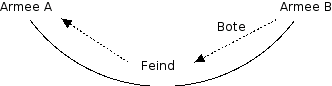
\includegraphics[width=80mm]{vs34.png}
		\end{center}
		\end{figure}
	\item Fehlermodell: Nachrichten k\"{o}nnen verloren gehen (Der Bote mu{\ss} durch die feindlichen Linien)
	\item Annahme: Es gibt ein Protokoll, dass mit $M$ Nachrichten Konsenz herstellt.\\
		\\
		Weil die Nachricht $M$ verloren gehen kann, das Protokoll aber sicherstellt, dass selbst dann Einigung erzielt wird, ist Nachricht $M$ nicht n\"{o}tig.\\
		\\
		$\Ra$ Es gibt ein Konsensprotokoll mit $M-1$ Nachrichten\\
		\\
		$\Ra$ Es gibt ein Konsensprotokoll mit $0$ Nachrichten\\
		\\
		Das ist ein Widerspruch!
\end{itemize}

\section{Verteilte Objekte und entfernter Aufruf}

\subsection{Teilproblem 1: Datentransport zwischen Client und Server}
Daten m\"{u}ssen zwischen Client und Server transportiert werden.
\begin{itemize}
	\item \textbf{Daten in Objekten:} Menge verkn\"{u}pfter Objekte. Attribute von Objekten im Speicher
	\item \textbf{Nachrichten:} Folge von Bytes
\end{itemize}
Notwendig ist die Umwandlung von ``Objekten'' in eine ``flache Darstellung'' (z.B. in eine Folge von Bytes). Verschiedene Rechner/Systeme stellen schon die elementaren Datentypen verschieden im Speicher dar. Die Darstellung im Speicher ist eine zur \"{U}bertragung ungeeignete Form.\\
\\
Generelle Methoden zur \"{U}bertragung:
\begin{enumerate}
	\item Umwandlung in ein externes Format. Umwandlung in dieses Format beim Senden und Empfangen.
	\item Werte werden im Format des Senders \"{u}bertragen. Empf\"{a}nger wandelt die Daten ggf. um.
\end{enumerate}
Oft m\"{u}ssen mehrere Werte gemeinsam \"{u}bertragen werden. Das Zusammenfassen zu einer Nachricht ist dann effektiver als die \"{U}bertragung in einzelnen Nachrichten. Diese Technik nennt man ``Marshalling'' (das ist: Die Umsetzung von strukturierten Datentypen in ein externes Format).\\
\\
Standardisierte Verfahren:
\begin{enumerate}
	\item Objektserialisierung in Java
	\item Datendarstellung in CORBA f\"{u}r Argumente und Ergebnisse entfernter Methodenaufrufe.\\
		\\
		CORBA: \textbf{C}ommon \textbf{O}bject \textbf{R}equest \textbf{B}roker \textbf{A}rchitecture.
\end{enumerate}
Marshalling wird von der Middleware ausgef\"{u}hrt. \"{U}blicherweise Umsetzung in Bin\"{a}r- oder Oktettdarstellung. (Evtl. XML wandelt in ``lesbares ASCII'' um).\\
\\
In CORBA hat man die folgenden Datentypen standardisiert: 15 elemtare Datentypen:\\
\\
\begin{tabular}{l|l}
	\textbf{Typ} & \textbf{Gr\"{o}{\ss}e} \\
		\hline
	short & 16 Bit \\
	long & 32 Bit \\
	float & 32 Bit \\
	double & 64 Bit \\
	char & \\
	boolean & \\
	octet & \\
	any & \\
\end{tabular} \\
\\
Zusammengesetzte Typen:\\
\\
\begin{tabular}{l|l}
	\textbf{Typ} & \textbf{Beschreibung} \\
		\hline
	Sequence & L\"{a}nge + Elemente\\
	String & L\"{a}nge + Elemente\\
	Array & Elemente in der gegebenen Reihenfolge. \\
	 & Anzahl der Elemente mu{\ss} fest und bekannt sein.\\
	Struct & Komponenten hintereinander
\end{tabular}
\\
\\
\\
In CORBA: Ausrichtung von Teilen auf 32-Bit-Grenzen. Typen werden nicht mit \"{u}bertragen, weil Sender und Empf\"{a}nger sich bei jeder Nachricht einig sind, welche Daten ausgetauscht werden. Die Spezifikation von Datentypen f\"{u}r den Austausch erfolgt in der \textbf{I}nterface \textbf{D}efinition \textbf{L}anguage (IDL).\\
\\
Beispiel:\\
\\
\texttt{
	struct Person \{\\
	$~\qquad$string name;\\
	$~\qquad$string place;\\
	$~\qquad$long year;\\
\};}\\
\\
Man verwendet einen Schnittstellencompiler. Dieser erzeugt aus den Beschreibungen der Datentypen in der IDL die Operationen f\"{u}r Marshalling und Unmarshalling.\\
\\
\textbf{Achtung:} Auch Verweise (Referenzen) auf Objekte treten als Daten auf. D.h. f\"{u}r entfernte Objekte mu{\ss} es ``eindeutige Bezeichner'' geben. Referenzen m\"{u}ssen unabh\"{a}ngig von Adressr\"{a}umen und Implementationen weitergegeben werden k\"{o}nnen.\\
\\
\textbf{Java Objektserialisierung}: Klasseninformationen, Methoden usw. k\"{o}nnen ggf. mit \"{u}bertragen werden oder m\"{u}ssen dem Empf\"{a}nger zur Verf\"{u}gung stehen. Aufbau ist rekursiv.\\
\\
Zwei Sichtweisen aufs Programmieren:
\begin{enumerate}
	\item Objektorientiertes Programmiermodell\\
		\\
		Um dieses Modell auf verteilte Systeme zu erweitern verwendet man \"{u}blicher Weise so etwas wie \textbf{R}emote \textbf{M}ethod \textbf{I}nvocation (RMI) \textit{(Achtung: 2 Arten von RMI, einmal das was Java macht und einmal das Konzept an sich selbst)}.\\
		\\
		\textit{Sichtweise:} ``Methoden \"{a}ndern Attribute''
	\item Ereignisorientiertes Programmiermodell\\
		\\
		Objekte erhalten Nachrichten \"{u}ber die Ereignisse von entfernten Objekten. Das ``System'' selbst soll Ereignisse herstellen k\"{o}nnen und dann Benachrichtigungen erzeugen.\\
		\\
		Mit so einem Konzept kann man dann ereignisorientiert programmieren. Man will auch in verteilten Systemen ereignisbasiert programmieren k\"{o}nnen.
\end{enumerate}
F\"{u}r beide F\"{a}lle ben\"{o}tigt man eine Schnittstellendefinition, in welcher nicht nur die Datentypen festgelegt sind, sondern auch die ``Parameter'' und ``Ergebnisse'' \textit{(In Anf\"{u}hrungszeichen weil von verschiedenen Programmiersprachen diese Begriffe anders verwendet werden)} und die Methodenaufrufe selbst.\\
\\
Methoden werden durch ihre Signatur festgelegt. Die Schnittstelle mu{\ss} Implementationsunabh\"{a}ngig festgelegt werden (Ausser man bleibt in einer Sprache). Daf\"{u}r wird wieder die IDL verwendet.\\
\\
Beispiel:\\
\\
\texttt{
	struct Person \{\\
	$~\qquad$string name;\\
	$~\qquad$string place;\\
	$~\qquad$long year;\\
\};}\\
\\
\texttt{
	interface PersonList \{\\
	$~\qquad$readonly attribute string listname;\\
	$~\qquad$void addPerson(in Person p);\\
	$~\qquad$void getPerson(in string name, out Person p);\\
	$~\qquad$long number();\\
\};}\\
\\
Parameter werden als ``Input'' oder ``Output'' deklariert, damit klar ist, wann Werte zwischen Aufrufer und Aufrufenden zu transportieren sind. Zeiger (als Referenz in Adressraum) d\"{u}rfen nicht als Parameter verwendet werden. Das ist sinnvoll, weil Adressen nur in einem Adressraum interpretierbar sind.\\
\\
Man kann \"{u}blicherweise nicht direkt auf Attribute von entfernten Objekten zugreifen, sondern nur mit GET- oder SET-Methoden. \\
\\
Man will Referenzen auf Objekte \"{u}bergeben k\"{o}nnen. Idee: Verwende global eindeutige Bezeichner f\"{u}r Objekte.\\
\\
\begin{tabular}{l|l|l|l|l}
	32 Bit & 32 Bit & 32 Bit & 32 Bit & \\
		\hline
	Internetadresse & Portnummer & Zeit & Objektnummer & Schnittstelle des entfernten Objekts \\
\end{tabular}

\subsubsection{Aufrufsemantik}
\begin{itemize}
	\item Vielleicht
	\item Mindestens einmal
	\item H\"{o}chstens Einmal
\end{itemize}
\begin{itemize}
	\item JAVA und CORBA: H\"{a}chstens einmal
	\item SUN-RPC: Mindestens einmal
\end{itemize}
 
 
\subsection{Begriff der ``idempotenten Opertation''}
Eine Operation hei�t idempotent wenn die zweimalige Ausf�hrung dasselbe
bewirkt, wie die einmalige Ausf�hrung.

\begin{itemize}
	\item Implementierung von RMI: Welche Teilprobleme werden gel\"{o}st?
	\item Entferntes Referenzmodul: Umsetzung lokaler Referenzen in entfernte Referenzen mittels einer Tabelle entfernter Objekte.
	\item Proxy: Spiegelt eine ``lokale Kopie''des entfernten Objekts vor.
	\item Das Proxy-Objekt verbirgt die Objekt-Referenz-Umsetzung. 
	\item Das Marshalling und Un-Marshalling: Senden und Empfangen von Nachrichten
	\item SKELETON: Implementiert die Methoden der entfernten Schnittstelle
\end{itemize}
Die SKELETON-Methoden werden \"{u}blicherweise nur einmal pro Klasse implementiert, und ein DISPATCHER verteilt die entfernten Aufrufe an die richtigen Objekte der Klasse.\\
\\
Wie werden die Klassen f�r PROXY und SKELETON erzeugt? Daf\"{u}r gibt es Schnittstellencompiler!!!\\
\\
Entfernte Aufrufe werden \"{u}blicherweise von eigenen Threads abgearbeitet, damit die Benutzung der entfernten Schnittstelle nicht zu zu starker Beeintr\"{a}chtigung beim Besitzer des benutzten Objektes f\"{u}hrt.\\ 
\\
Implementierung von entfernten Objekten m\"{u}ssen THREAD-SAFE sein. Ein entferntes Objekt steht nur in einem Prozess zur Benutzung zur Verf\"{u}gung. Damit nicht st\"{a}ndig f\"{u}r alle entfernten Objekte die zugeh\"{o}rigen Prozesse laufen m\"{u}ssen, erlaubt man ``passive Objekte'' die von einem Aktivator gestartet werden.\\
\\ 
Persistente Objekte: Die Existenz ist gesichert \"{u}ber die Beendigung von Prozessen hinweg. In CORBA gibt es den Persistant Object Service. Der benutzt Festplatten f\"{u}r die Zwischenspeicherung. In verteilten Systemen mu{\ss} man Objekte mit verteiltem Garbage-Collection aufr\"{a}umen.
 
\subsubsection{Ereignisse und Benachrichtigungen}
Ziel: Objekt reagiert auf �nderungen in einem andern Objekt.\\
\\
Die Situation ist durch folgende Eigenschaften oft gekennzeichnet: Benachrichtigungen sind typischerweise asynchron.\\
\\ 
Man wei{\ss} nie, wann welches Ereignis stattfind bzw. wann es gemeldet wird.  Heterogenit\"{a}t (Einsatz verschiedenster Systeme) ist erw\"{u}nscht.\\
\\
Modellvorstellung: Publish-Subscribe Modell
\begin{itemize}
	\item Publisher: In Objekten geschehen Ereignisse. Die Objekte geben bekannt, dass sie �ber diese Ereignisse benachrichtigen k\"{o}nnen.
	\item Subscriber: Objekte geben bekannt, dass sie �ber bestimmte Ereignisse benachrichtig werden wollen.
\end{itemize}
Ereignisse haben Attribute
\begin{itemize}
	\item Namen des Erzeugerobjekts
	\item Operation die das Ereignis ausl�ste
	\item Parameter solcher Operationen
	\item Zeit
\end{itemize}
Konzeptidee:
\begin{itemize}
	\item Trenne den Publisher und den Subscriber um getrennte Entwicklung zu erm\"{o}glichen.
	\item Begrenze dadurch auch die Arbeit, die die Subscriber f\"{u}r den Publisher bedeuten.
	\item Richte einen Ereignisdienst ein mit Beobachterobjekten.
	\item Bei Benachrichtigungen kann man verschiedene Garantieanforderungen stellen.
	\item Realisierung mit IP-Multicast.
	\item Keinerlei Auslieferungs- oder Reihenfolgegarantie.
	\item Beim RELIABLE-Multicast w�re eine Alles- oder Nichts-Semantik realisiert.
	\item Eventuell will man Echtzeitanforderungen erf\"{u}llen. 
	\item In synchronen Systemen gibt es Multicast-Protokolle mit Echtzeitgarantie.
	\item Zuverl\"{a}ssigkeit und Reihenfolgegarantie. Damit kann man Garantien in ereignisbasieren System erbringen. 
\end{itemize}
Beobachter haben verschiedenste Aufgaben:
\begin{itemize}
	\item ``Weitergabe'', eventuell mit Garantie
	\item ``Filterung'': Nur die ``interessanten'' Nachrichten werden weitergeleitet
	\item ``Mustererkennug'': Kombinationen von Ereignissen f\"{u}hren zur Benachrichtigung
	\item ``Mailbox'': Abholdienst, falls der Subscriber selten aktiv ist. 
\end{itemize}
 
\subsection{Das verteilte Objektmodell}
\begin{itemize}
	\item \textbf{Entfernte Objektreferenz:} Objekte k\"{o}nnen Methoden eines entfernten Objektes aufrufen, wenn sie eine Objektreferenz auf dieses Objekt besitzen.
	\item \textbf{Entfernte Schnittstelle:} Jedes entfernte Objekt hat eine entfernte Schnittstelle, die angibt, welche seiner Methoden aufgerufen werden k\"{o}nnen.
\end{itemize}
(Siehe Aush\"{a}ndigungen)\\
\\
Entfernte Objektreferenzen:
\begin{itemize}
	\item Identifikation, die innerhalb eines verteilten Systems ein entferntes Objekt eindeutig identifiziert.
	\item \textbf{Achtung:} Man will Objekte eventuell verschieben, ohne dass man die Objektreferenzen \"{a}ndert. 
	\item \textbf{Achtung:} Man mu{\ss} davon ausgehen, dass entfernte Methodenaufrufe fehlschlagen (z.B. Netzwerkausfall, Serverausfall). Deswegen sollten Aufrufer (Clients) in der Lage sein, Exceptions zu verarbeiten die im Fehlerfall auftreten.
\end{itemize}
Probleme beim entfernten Methodenaufruf:
\begin{itemize}
	\item Anforderungsnachrichten k\"{o}nnen verloren gehen.\\
		\\
		A) Wiederhole Anforderungsnachrichten
	\item Anforderungen an den Server gehen mehrfach ein.\\
		\\
		B) Filter Duplikate aus
	\item Ergebnisnachrichten gehen verloren.\\
		\\
		C) Speichere die Folge der Ergebnisnachrichten und wiederhole ggf. verlorene Nachrichten, ohne dass die eigentliche Operation auf dem Server ein zweites Mal gemacht wird.
\end{itemize}
Aufrufsemantik:
\begin{itemize}
	\item Vielleicht: Weder A noch B noch C
	\item Mindestens einmal: A $\quad$ B nicht $\quad$ C nicht\\
		\\
		(Es wird schon auf eine Ergebnisnachricht gewartet, zumindest eine Zeitlang)
	\item H\"{o}chstens einmal: A und B und C\\
		\\
		Es wird davon ausgegangen, dass der Server abst\"{u}rzen kann. Daher kann ein entfernter Methodenaufruf keine ``garantiert genau einmal'' Forderung erf\"{u}llen.
\end{itemize}


\section{Verteilte Dateisysteme}
Verteilte Dateisysteme bilden die Grundlagen f\"{u}r viele andere verteilte Dienste.\\
\\
Anforderungen:
\begin{itemize}
	\item \textbf{Zugriffstransparanz:} Client Programme m\"{u}ssen nicht darauf R\"{u}cksicht nehmen, dass sich die benutzten Dateien in einem verteilten Dateisystem befinden. Sie benutzen die gleichen Aufrufe.
	\item \textbf{Orts- und Mobilit\"{a}tstransparenz:} Der Ort, an welchem Daten physikalisch liegen, darf sich \"{a}ndern, ohne dass Benutzer darauf R\"{u}cksicht nehmen m\"{u}ssen. Die Benutzer d\"{u}rfen ihren Ort auch \"{a}ndern.
	\item \textbf{Skalierungstransparenz:} Inkrementelles Wachstum erlaubt effektive Behandlung gr\"{o}{\ss}erer Datenmengen, gro{\ss}er Benutzermengen, u.s.w.
\end{itemize}
Nebenl\"{a}ufige Benutzung von Dateien soll m\"{o}glich sein. Eventuell will man sogar nebenl\"{a}ufige \"{A}nderungen von Dateien. (Oft wird kein globales hartes Sperrkonzept eingesetzt, weil die Performance dann zu stark leidet!).
\begin{itemize}
	\item \textbf{Replikation} oder teilweise Replikation soll m\"{o}glich sein (Caching).
	\item \textbf{Heterogenit\"{a}t} von Hardware und Betriebssystemen soll unterst\"{u}tzt werden.
	\item \textbf{Fehlertoleranz}, d.h. z.B. Verlust von Nachrichten oder Absturz von Prozessen soll toleriert werden.\\
		\\
	Verwende z.B. idempotente Dateioperationen. Verwende ``zustandslose'' Server. Die Idee dabei ist, dass ein Server sich nach Absturz neu starten l\"{a}{\ss}t, und sich danach so verh\"{a}lt als sei er nicht abgest\"{u}rzt. Realisierung mit LOG-Dateien und COMMIT-Records.
	\item \textbf{Konsistenz:} Eine Forderung k\"{o}nnte sein: Ein-Kopie-Aktualisierungssemantik: ``Alle Clients sehen das, was sie sehen w\"{u}rden, wenn es die Datei nur einmal g\"{a}be.''\\
		\\
		Problem: \"{A}nderungen von Dateibereichen m\"{u}ssen in allen Repliken gemacht werden.
	\item \textbf{Sicherheit und Zugriffskontrolle:} Authentifizierung, Signaturen, Verschl\"{u}sselung
	\item \textbf{Effizienz:} Es sollen die gleichen Dienste erbracht werden, wie in einem klassischen Dateisystem. Man m\"{o}chte ein hohes Ma{\ss} an Leistung (Durchsatz).
\end{itemize}
Verteilte Dateisysteme werden oft mit Hilfe eines ``Flachen Dateidienstes'' implementiert. Verwendung einer einfachen Schnittstelle mit wenigen der definierten Operationen. 
\begin{itemize}
	\item Der flache Dateidienst verwendet UFID (Unique File Identifier) innerhalb des verteilten Dateisystems.
	\item Die Operationen (READ, WRITE, CREATE, DELETE, GETATTRIB Und SETATTRIB) werden mit Hilfe von Remote-Procedure-Calls implementiert.
	\item Um Dateinamen verweden zu k\"{o}nnen wird zum flachen Dateidienst ein Verzeichnisdienst hinzugef\"{u}gt. Dieser realisiert die Umsetzung von Namen $\leftrightarrow$ UFID.
	\item Das Client-Modul stellt den Applikationen die \"{u}bliche Benutzung (API) zur Verf\"{u}gung.
\end{itemize}
Zu den Operationen mit Ausnahme von CREATE sind die Operationen des flachen Dateidienstes idenpotent spezifiziert. Die Verwendung der ``Mindestens Einmal'' Semantik f\"{u}r die Implementation der RPC ist hinreichend.\\
\\
Selbst CREATE ist nicht kritisch. Jeder Aufruf erzeugt zwar eine neue ``Datei'' (UFID) aber die Eindeutigkeit ist gew\"{a}hrleistet. Eventuell mu{\ss} der Server manchmal ungenutzte UFIDs aufr\"{a}umen.\\
\\
Server k\"{o}nnen leicht zustandslos implementiert werden. Ein Server hei{\ss}t zustandslos, wenn er nach Absturz problemlos wieder gestartet werden kann.\\
\\
Vorsicht: Das klassische UNIX-Dateisystem entspricht diesem modell in wesentlichen Punkten nicht!
\begin{itemize}
	\item ``OPEN'' und ``CLOSE'' in UNIX erfordern einen Zustand. 
	\item Bei ``READ'' und ``WRITE'' Operationen gibt es eine File-Position, die einen Zustand entspricht.
	\item READ und WRITE Operationen in UNIX sind nicht idenpotent.
\end{itemize}
Zugriffskontrolle erfolgt \"{u}blicherweise auf dem Server. Sicherung gegen gef\"{a}lschte Identifikationen und gef\"{a}lschte UFIDs ist n\"{o}tig. Das Ergebnis einer Zugriffs\"{u}berpr\"{u}fung wird dem Client mitgeteilt. Das Ergebnis wird nicht beim Server gespeichert weil sonst die Zustandslosigkeit schwer zu realisieren w\"{a}re.\\
\\
Eine Methode w\"{a}re:
\begin{itemize}
	\item Bei der Umwandlung Name $\rightarrow$ UFID wird an den Client zur\"{u}ckgegeben, was der Aufrufer alles mit der Datei darf.
\end{itemize}
Die Schnittstelle zum Verzeichnisdienst:
\begin{itemize}
	\item Alle Methoden sind idenpotent spezifiziert.
	\item Um hierarchische Dateisysteme abzubilden, benutzt man mehrfach die Umsetzung Name $\rightarrow$ UFID.
		\begin{itemize}
			\item abc/xyz/java.com
			\item ``abc'' $\rightarrow$ UFID(abc)
			\item Dann ist UFID(abc), suche nach xyz
			\item Dann ist UFID(abc/xyz), suche nach java.com
		\end{itemize}
\end{itemize}
\subsection{Eine Beispimplementation (NFS)} ...f\"{u}r ein verteiltes Dateisystem:
SUN-NFS (Siehe ausgeh\"{a}ndigtes Blatt)\\
\\
Ein m\"{o}gliches NFS-Szenario
\begin{itemize}
	\item T READ soll hei{\ss}en in der Datei wird das Zeichen an der ersten Position gelesen. Der Aufruf erfolgt zur Zeit $T$.
	\item T WRITE(C) Ein Client ruft zur Zeit $T$ die Schreiboperation auf, die Zeichen C an die erste Position der Datei schreibt.
	\item OPEN und CLOSE teilt dem lokalen Dateisystem das \"{u}bliche mit
\end{itemize}
Bl\"{o}cke im Client-Cache werden nur beim COMMIT bzw. hier ``CLOSE'' zum Server \"{u}bertragen. Verwende $t=5s$ als Aktualisierungsschranke.\\
\\
$(C,t_m)$ auf dem Server hei{\ss}t: Dateiinhalt ist $C$ und wurde zur Zeit $t_m$ auf dem Server das letzte Mal ge\"{a}ndert.

\subsection{Ein weiteres verteiltes Dateisystem (AFS)}
AFS: Andrew-File-System
\begin{itemize}
	\item Gesamte Dateien werden vom Server zum Client \"{u}bertragen und dort gecached. Der Cache im Client ist permanent, d.h. er \"{u}berlebt den Absturz oder Neustart eines Client-Computers. Die Idee ist, dass so vielleicht viele Dateien benutzt werden k\"{o}nnen, ohne dass weitere Netzlast entsteht.
	\item Bei ``Open'' wird festgestellt, ob man mit einer lokalen Kopie arbeiten kann.
	\item Wie wird die Aktualit\"{a}t von Kopien gew\"{a}hrleistet?? Wie nahe kommt man an die Ein-Kopie-Aktualisierungssemantik?
	\item Bei der \"{U}bertragung einer Kopie vom Server zum Client stellt der Server dem Client ein Callback-promise-Token zur Verf\"{u}gung. Der Server ``verspricht'' dem Client, ihn \"{u}ber Aktualisierungen zu informieren.
	\item Zustand des promise-Tokens auf dem Client
	 	\begin{itemize}
			\item ``VALID'' bei Zustellung
			\item ``CANCELLED'' wird gesetzt, wenn der Server \"{u}ber eine Aktualisierung berichtet
	 	\end{itemize}
\end{itemize}
\textit{Weiteres siehe Ausgeh\"{a}ndigtem.} Falls bei ``OPEN'' das Token den Wert ``Cancelled'' hat, wird eine neue Kopie geholt. Bei Neustart des Clients mu{\ss} er f\"{u}r alle Dateien im Cache pr\"{u}fen, ob er CALLBACKs verpa{\ss}t hat. D.h. die Callback-promises m\"{u}ssen aktualisiert werden. Das sch\"{u}tzt gegen den Verlust von Callback-Nachrichten. Auf diese Weise kann die Ein-Kopie-Aktualisierungssemantik nicht garantiert werden. Aber man versucht, sich ihr zu n\"{a}hern bei gleichzeitig sehr niedriger Netzlast (Netzlast nur bei OPEN und CLOSE\textit{, viel niedriger als bei NFS}).\\
\\
Erstaunlicherweise verh\"{a}lt sich das AFS in der Praxis relativ gut. Warum ist das so?
\begin{itemize}
	\item Weil viele Dateien relativ klein sind, kann der Client tats\"{a}chlich ganze Dateien cachen.
	\item Die meisten Dateien werden nur gelesen und sehr sehr selten ge\"{a}ndert (Performance besser als NFS wegen geringer Netzlast).
	\item Dateien die sowohl viel gelesen als auch geschrieben werden, werden oft nur von einem Benutzer benutzt (Performance besser als NFS wegen geringer Netzlast).
	\item Dateien werden oft geh\"{a}uft hintereinander von einem Benutzer (auf einem Client) benutzt. 
\end{itemize}
Problem: Datenbanken passen \"{u}berhauptnicht in dieses Bild. Bei Datenbanken sind Korrektheit und nebenl\"{a}ufige Benutzung unverzichtbar.

\section{Transaktionen und Nebenl\"{a}ufigkeitskontrolle}
Verwende folgende Sichtweise:
\begin{itemize}
	\item Ein Server stellt mehrere Objekte bereit.
	\item Eine Transaktion wird von einem Client angefordert (spezifiziert) und beeinflu{\ss}t im allgemeinen mehrere Objekte.
\end{itemize}
Vom Server soll die folgende Garantie erbracht werden:
\begin{itemize}
	\item Die gesamte Transaktion wird durchgef\"{u}hrt...
	\item ...oder die Transaktion hat keine Wirkung (und es wird dem Client mitgeteilt, dass die Transaktion fehlschlug)
\end{itemize}
Transaktionen sollen nebenl\"{a}ufig ausgef\"{u}hrt werden! Damit Abst\"{u}rze des Servers toleriert werden, werden alle Objekte presistent (dauerhaft) gespeichert. Clients fordern, dass eine Folge von Schritten, die eine Transaktion bilden, atomar ausgef\"{u}rt werden.  Strikte Hintereinanderausf\"{u}hrung ist zu ineffektiv: Man m\"{o}chte die Teilschritte verzahnen.\\
\\				  
\textbf{Isolationsbedingung:} Jede Transaktion ist so durchzuf\"{u}hren, dass sie durch andere, nebenl\"{a}ufig ablaufende Transaktionen, nicht gest\"{o}rt wird. Zwischeneffekt einer Transaktion sind unsichtbar f\"{u}r alle anderen Transaktionen.\\
\\
Es gibt zwei Probleme bei nebenl\"{a}ufiger Ausf\"{u}hrung \textit{(siehe Aush\"{a}ndigungen: Lost Update, Problem der inkonsistenten Abrufe)}.\\
\\
\"{U}blicherweise fordert man von einem Transaktionssystem die ``serielle \"{A}quivalenz'' wenn man mehrere Transaktionen ausf\"{u}hrt. Das Ergebnis einer nebenl\"{a}ufigen verzahnten Ausf\"{u}hrung wird als korrekt betrachtet, falls es eine Hintereinanderausf\"{u}hrung der Transaktion gibt, die zum selben Ergebnis f\"{u}hrt.\\
\\
Beispiel:
\begin{tabular}{cc|cc}
	\textbf{Schritt} & \textbf{Transaktion T} & \textbf{Schritt} & \textbf{Transaktion U} \\
	\hline 
	T1 & x = read(i) & U1 & y = read(j) \\
	T2 & write(i,10) & U2 & write(j,30) \\
	T3 & write(j,20) & U3 & z = read(i)\\
\end{tabular}\\
\\
\\
Am Anfang sei der Wert von i = 1 und j = 2\\
\\
Reihenfolge T dann U:\\
\\
\begin{tabular}{c|c|c}
	\textbf{Schritt} & \textbf{Transaktion} & \textbf{Wert} \\
	\hline 
	T1 & x = read(i) & x = 1 \\ 
	T2 & write(i, 10) & i = 10 \\
	T3 & write(j, 20) & j = 20 \\
	U1 & y = read(j) & y = 20 \\
	U2 & write(j,30) & j = 30 \\
	U3 & z = read(i) & z = 10 \\
\end{tabular}\\
\\
Gesamtwirkung: i = 10, j = 30, x = 1, y = 20, z = 10\\
\\
Reihenfolge U dann T:\\
\\
\begin{tabular}{c|c|c}
	\textbf{Schritt} & \textbf{Transaktion} & \textbf{Wert} \\
	\hline 
	U1 & y = read(j) & y = 2 \\
	U2 & write(j,30) & j = 30 \\
	U3 & z = read(i) & z = 1 \\
	T1 & x = read(i) & x = 1 \\ 
	T2 & write(i, 10) & i = 10 \\
	T3 & write(j, 20) & j = 20 \\
\end{tabular}\\
\\
\\
Gesamtwirkung: i = 10, j = 20, x = 1, y = 2, z = 1\\
\\
Eine nicht seriell \"{a}quivalentes Interleaving:\\
\\
\begin{tabular}{cc|cc|c}
	\textbf{Schritt} & \textbf{Transaktion T} & \textbf{Schritt} & \textbf{Transaktion U} & \textbf{Wert} \\
	\hline 
	T1 & x = read(i) & & & x = 1 \\ 
	T2 & write(i, 10) & & & i = 10 \\
	& & U1 & y = read(j) & y = 2 \\
	& & U2 & write(j,30) & j = 30 \\
	T3 & write(j, 20) & & & j = 20 \\
	& & U3 & z = read(i) & z = 10 \\
\end{tabular}\\
\\
\\
Gesamtwirkung: i = 1, j = 20, x = 1, y = 2, z = 10\\
\\
Wie kann man sicherstellen, dass die Verzahnung, die man w\"{a}hlt, seriell \"{a}quivalent ist? Idee: Konflikterzeugende Operation.\\
\\	
Ein Operationspaar erzeugt einen Konflikt $\Leftrightarrow$ Die kombinierte Wirkung h\"{a}ngt von der Reihenfolge ab.\\
\\
\textbf{Beispiele:}
\begin{itemize}
	\item read(a); read(a) kein Konflikt
	\item read(a); write(a,5) Konflikt
	\item write(a,5); write(a,10) Konflikt
\end{itemize}
Wenn man Transaktionen so ausf\"{u}hrt, dass alle konflikterzeugenden Operationspaare in der gleichen Reihenfolge ausgef\"{u}hrt werden (d.h. wenn man einmal zuerst die Operation von Transaktion U gemacht hat, dann bei Konflikt immer erst die Operation von U) dann ist die Ausf\"{u}hrung seriell \"{a}quivalent.\\
\\
Wie sorgt man daf\"{u}r, dass nicht gegen Konfliktregeln versto{\ss}en wird:
\begin{itemize}
	\item Kontrolliere den Zugriff auf Objekte durch Sperren! (LOCKs)
\end{itemize}
Vorsicht: Man darf Sperren nicht zu fr\"{u}h freigeben. Eine korrekte Vorgehensweise ist das 2-Phasen-Sperren.
\begin{itemize}
	\item Sammelphase: Sperren anfordern
	\item Freigabephase: Sperren freigeben
\end{itemize}
Probleme bei Sperren: 
\begin{itemize}
	\item Deadlocks
	\item Hocher Verwaltungsaufwand
	\item Geringer Durchsatz
\end{itemize}
Deadlocks sind hier nicht so problemantisch, weil das Transaktionssystem die M\"{o}glichkeit hat Transaktionen abzubrechen!\\
\\
\textbf{Idee:} Mache bereits eingetretene Wirkung r\"{u}ckg\"{a}ngig. Aber, der Abburch von Transaktionen kann zu zus\"{a}tzlichen Problemen f\"{u}hren: \textit{Siehe Aush\"{a}ndigung ``Dirty-Read''.}
\begin{itemize}
	\item Sperren m\"{u}ssen gehalten werden, bis ``COMMIT'' oder ``ABORT'' feststeht.
	\item Anderenfalls kann das R\"{u}ckg\"{a}ngigmachen, da dabei ``WRITE-Operationen'' vorkommen, zu Problemen f\"{u}hren.
\end{itemize}
Da das strikte Vermeiden von Konflikten kann die Performance stark herabsetzt. Man kann eine andere Vorgehensweise verwenden: ``Optimistische Vorgehensweise''. F\"{u}hre die Transaktionen an Versuchsszenarien der Objekte aus. Danach pr\"{u}fte auf Konfliktfreiheit und schreibe erst dann fest (Festschreiben entspricht COMMIT)\\
\\
Bisher lagen alle Objekte, die von einer Transaktion betroffen wurden, auf einem Server. \textit{Bei den verteilten Transaktionen sieht dies anders aus.}
\subsection{Verteilte Transaktionen}
Die von einer Transaktion betroffenen Objekte werden von mehreren Servern verwaltet. Eventuell kann eine Transaktion auch Unter-Transaktionen starten \textit{(siehe Aush\"{a}ndigung ``Verteilte Transaktionen'')}.\\
\\
Problem:
\begin{itemize}
	\item Die Atomarit\"{a}t einer Transaktion (alles oder nichts) mu{\ss} gesichert bleiben. 
	\item Server k\"{o}nnen abst\"{u}rzen!
	\item Nachrichten k\"{o}nnen verloren gehen!
	\item Wichtigster Punkt: Es mu{\ss} Einigkeit hergestellt werden, ob 
		\begin{itemize}
			\item festschreiben...
			\item ...oder abbrechen
		\end{itemize}
\end{itemize}
L\"{o}sungsansatz: Atomare Commit Protokollei mit Hilfe eines Koordinators. (Vorher eventuell Wahl eines Koordinators)\\
\\
Aufgaben des Koordinators:
\begin{itemize}
	\item Beim Start einer Transaktion
		\begin{itemize}
			\item Client teilt dem Koordinator mit, dass er eine Transaktion startet.
			\item Der Koordinator gibt dem Client eine TID (Transaktionsidentifikation) zur\"{u}ck und startet die Transaktionsverwaltung. Die TID ist eindeutig im verteilten System.
		\end{itemize}
	\item W\"{a}hrend der Ausf\"{u}hrung
		\begin{itemize}
			\item Jeder Server, der ein Objekt verwaltet, das von einer Transaktion betroffen ist, meldet dem Koordinator, dass er an der Transaktion beteiligt ist (``JOIN''-Operation).
		\end{itemize}
\end{itemize}
Koordinator f\"{u}rt f\"{u}r jede Transaktion eine liste aller Teilnehmer. Jeder Teilnehmer hat eine Referenz auf den Koordinator. Alle diese Listen sind permanent (absturzgesichert) gespeichert!\\
\\
Wenn die Transaktion beendet werden soll:
\begin{itemize}
	\item Client fordert mit ``CLOSE-TRANSACTION'' den Koordinator auf, das Commit-Protokoll auszuf\"{u}hren. 
	\item Eventuell gibt es schon vorher irgendeinen Teilnehmer der ``ABORT-TRANSACTION'' vom Koordinator anfordert.
\end{itemize}
\textit{(Siehe Aush\"{a}ndigung: ``Eine verteilte Banking-Transaktion'')}.

\subsection{Commit-Protokolle}
\subsubsection{Ein-Phasen Commit-Protokoll}
Ein einfaches (unzureichendes) Ein-Phasen Commit-Protokoll:
\begin{itemize}
	\item Koordinator entscheidet und fordert alle Teilnehmer auf, die Transaktion festzuschreiben oder abzubrechen.
	\item Anforderung wiederholen, bis eine Best\"{a}tigung von allen Teilnehmern erhalten ist.
Problem: Wenn ein Server nicht festschreiben kann, kann er bei diesem Protokoll keinen Abbruch veranlassen! Gr\"{u}nde daf\"{u}r k\"{o}nnen sein: Die lokale Nebenl\"{a}ufigkeitskontrolle hat einen Deadlock festgestellt.
\end{itemize}
\begin{figure}[htbp]
\begin{center}
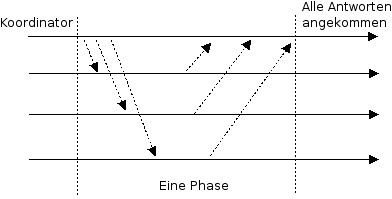
\includegraphics[width=100mm]{vsx01.png}
\end{center}
\end{figure}
Beim optimistischen Verfahren kann es sein, dass konflikterzeugende Operationen den Abbruch als Konfliktl\"{o}sung verlangen. Auch das Erkennen eines Serverabsturzes kann nicht verwendet werden.\\
\\
Abhilfe: Zwei-Phasen Commit-Protokoll

\subsubsection{Zwei-Phasen Commit-Protokoll}
Anforderungen:
\begin{itemize}
	\item Wenn ein Teilnehmer Abbruch verlangt, mu{\ss} abgebrochen werden.
	\item Wenn Konsens \"{u}ber Festschreiben besteht, m\"{u}ssen alle festschreiben.
	\item Wenn Server abst\"{u}rzen, soll das die Atomarit\"{a}t nicht gef\"{a}hrden.
\end{itemize}
Phasen:
\begin{enumerate}
	\item \textbf{Phase (Abstimmungsphase):} Unter den Teilnehmern wird per Abstimmung festgestellt, ob festgeschrieben oder abgebrochen werden soll.
		\begin{itemize}
			\item Teilproblem: Stimmt ein Teilnehmer f\"{u}r ``festschreiben'', mu{\ss} er in der Lage sein festzuschreiben. Er darf noch nicht festgeschrieben haben.
			\item Vorgehensweise: Bevor ein Teilnehmer mit ``festschreiben'' antwortet, sichert er seine Stimme im permanenten Speicher zusammen mit den festzuschreibenden Werten. \\
				\\
				Die Transaktion hat bei diesem Teilnehmer den Zustand ``vorbereitet zum Festschreiben'' (``PREPARED'').
		\end{itemize}
	\item \textbf{Phase (Mitteilungsphase):} Der Koordinator teilt allen Teilnehmern das Ergebnis der Abstimmung mit. Die Teilnehmer f\"{u}hren es aus \textit{(festschreiben oder abbrechen)}.
\end{enumerate}
\subsubsection{Fehlermodell:}
\begin{itemize}
	\item Verlust von Nachrichten
	\item Absturz von Servern
	\item Server k\"{o}nnen neugestartet werden und ihre Aufgabe mithilfe des permanenten Speichers fortf\"{u}hren
	\item Keine Zeitschranken
\end{itemize}
\textit{Weiteres siehe Aush\"{a}ndigungen}. Das Protokoll hat ein Problem, wenn Teilnehmer, die im unsicheren Zustand sind, den Koordinator nicht erreichen. Eventuell kann man anderen Teilnehmer fragen. Falls ein Teilnehmer die Entscheidung des Koordinators kennt, darf er sie anderen mitteilen.

\subsection{Bemerkungen zur Nebenl\"{a}ufigkeitsktontrolle bei Verteilten Systemen}
Jeder Server f\"{u}rt f\"{u}r seine Objekte lokal eine Nebenl\"{a}ufigkeitsktontrolle durch (d.h. lokal erreicht man serielle \"{A}quivalenz).\\
\\
$\alpha: a, B \qquad \beta: b, B$\\
\\
Das reicht nicht aus, um global serielle \"{A}quivalenz zu sichern.\\
\\
Eine M\"{o}glichkeit: Benutzung von Sperren im gesamten verteilten System. Vorsicht: Jetzt ist es viel schwieriger Deadlocks festzustellen, weil man nicht so leicht eine Momentaufnahme (Snapshot) machen kann um die ``Situation zu einem Zeitpunkt'' einzufangen.\\
\\
Es kann zu ``Phantom Deadlocks'' kommen, das sind Deadlocks, die in Wirklichkeit nicht da sind.\\
\\
Die Probleme f\"{u}hren dazu, dass man ungern globale Sperren verwendet. Besser: Global optimistische Vorgehensweise. Ein Koordinator ist f\"{u}r die Feststellung und L\"{o}sung von Konflikten verantwortlich. 

\section{Replikation}

\begin{itemize}
	\item Aufgabe: Hohe Verf\"{u}gbarkeit von Daten und Leistungsverbesserung.
	\item Ansatz: Daten werden auf mehreren Servern gehalten und zur Verf\"{u}gung gestellt.
	\item Forderung: Replikationstransparenz. Die Clients sollen nicht erkennen, dass mehrere physikalische Kopien existieren. Jedes Objekt gibt es als ``logisches Objekt'' nur einmal.
\end{itemize}
Wenn man Dienste repliziert, mu{\ss} die spezifizierte Korrektheit f\"{u}r den reguliertem Dienst weiter eingehalten werden. (Was immer das hei{\ss}en mag!)\\
\\
Systemmodell asynchrones System:
\begin{itemize}
	\item Nur Prozessabst\"{u}rze werden ber\"{u}cksichtigt.
	\item Keine Netwerkunterbrechungen und kein Nachrichtenverlust.
\end{itemize}
Replikenmenge (RM) verwalten eine einzelne Replik. Die RM f\"{u}hren alle Operationen ``wiederherstellbar'' aus. D.h. die Repliken \"{u}berstehen Abst\"{u}rze.\\
\\
Anforderungen von Clients werden \"{u}ber ein Frontend (FE) an die RM geleitet. Dabei sind die FE zusamemen mit den RM daf\"{u}r verantwortlich, Replikationstransparenz zu gew\"{a}hrleisten.\\
\\
Eine Replikation wird in 5 Phasen unterteilt:
\begin{enumerate}
	\item Das FE sendet die Anforderung an ein oder alle RM.
	\item Koordination: Die RM koordinieren die Reihenfolge, in der die Anforderungen ausgef\"{u}hrt werden (oder sie einigen sich auf Abbruch).\\
		\\
		An die Reihenfolgen stellt man oft gewisse Anforderungen. Eine Forderung ist z.B. die Forderung, dass FIFO Reihenfolge eingehalten wird. Genauer hei{\ss}t das: Wenn ein Frontend Anforderung $r$ vor $r'$ absetzt, verarbeitet jeder korrekte RM $r$ vor $r'$ sofern er $r'$ verarbeitet. 
		\begin{figure}[htbp]
		\begin{center}
		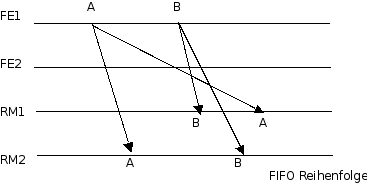
\includegraphics[width=70mm]{vsx03.png}
		\end{center}
		\end{figure}
		\begin{figure}[htbp]
		\begin{center}
		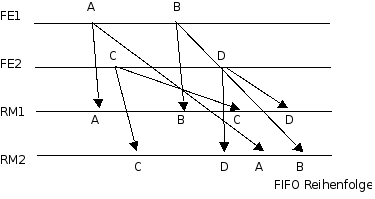
\includegraphics[width=70mm]{vsx04.png}
		\end{center}
		\end{figure}
		Vorsicht: Die FIFO-Garantie sichert noch keine Ein-Kopie-Aktualisierungs-Semantik.
	\item Die RM f\"{u}hren die Anforderungen aus (ggf. versuchsweise).
	\item Einigung: Die RM einigen sich dar\"{u}ber, welche Anforderungen festgeschrieben werden. (Und es wird ggf. festgeschrieben).
	\item Antwort: Ein oder mehrere RM antworten dem Frontend!
\end{enumerate}
Eventuell wird dem FE schon fr\"{u}her mitgeteilt, ob seine Anforderung ausgef\"{u}hrt wird oder nicht.\\
\\
Damit alle RM wissen, wer bei Koordinationsvorg\"{a}ngen beteiligt ist, wird ein Gruppenmitgliedsschaftdienst eingef\"{u}hrt! Beitrit und Austritt von Mitgliedern und Gruppenkommunikation werden damit realisiert.\\
\\
Eine Aufgabe des Gruppenmitgliedsschaftdienstes ist es ``Gruppenansichten'' zu verwalten und zu verteilen.\\
\\
Gruppenansicht (VIEW) ist eine Liste der aktuellen Gruppenmitglieder. Identifikation von Mitgliedern durch eine global eindeutig Prozessdienstidentifikation. Beim Aus- oder Eintritt von Mitgliedern wird eine neue Ansicht erzeugt.
\begin{figure}[htbp]
\begin{center}
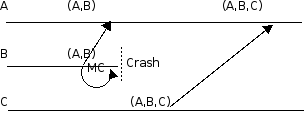
\includegraphics[width=70mm]{vsx05.png}
\end{center}
\end{figure}
\textit{Weiteres siehe Aush\"{a}ndigung.}

\subsection{2 Arten Daten bzw. Dienste zu replizieren}
\begin{enumerate}
	\item Art: Passive (Prim\"{a}r/Backup)-Replikation. (Siehe Aush\"{a}ndigungen).
	\item Art: Namensdienste / Verzeichnisdienste
\end{enumerate}

\section{Namensdienste}
Namen verweisen auf unterschiedlichste Ressourcen (Computer, entfernte Objekte, Dateien, Dienste...). Namen erleichtern Nutzung und Kommunikation. Beispiel: URL f\"{u}r WEB-Zugriffe.\\
\\
Namensdienste setzen dann den Namen in die Objektreferenz um. Beispiel: DNS
\begin{itemize}
	\item Domain-Name $\rightarrow$ Attribute des Hosts, z.B. IP, Host-Typ
\end{itemize}
CORBA:
\begin{enumerate}
	\item Naming Service
		\begin{itemize}
			\item Name eines entfernten Objektes $\rightarrow$ Objektverweis
		\end{itemize}
	\item Trading Service
		\begin{itemize}
			\item Name eines entfernten Objektes $\rightarrow$ Objektverweis + Attribute
		\end{itemize}
\end{enumerate}
Namen sind oft spezifisch f\"{u}r Dienste.
\begin{itemize}
	\item Dateinamen im Dateisystem 
	\item Prozess-ID im Betriebssystem
	\item Benutzername auf einem Rechner
	\item \textit{E-Mail Adressen}
	\item \textit{usw...}
\end{itemize}
Die Namen werden nur im Kontext dieses Dienstes verwendet.\\
\\
Aufgaben und Anforderungen an Namensdienste:
\begin{itemize}
	\item Verwaltung mehrerer Kontexte
	\item Aufl\"{o}sung von Namen, d.h. die Umsetzung Name $\rightarrow$ Attribute
	\item Erstellen und L\"{o}schen von Bindungen Name $\leftrightarrow$ Attribute
	\item Verwaltung von Namen \"{u}ber Systemgrenzen hinweg
	\item Verwaltung sehr gro{\ss}er Mengen von Namen	
	\item Der Dienst soll \"{A}nderungen der Implementation und Komponenten \"{u}ber lange Zeit \"{u}berstehen
	\item Der Dienst mu{\ss} h\"{o}chst verf\"{u}gbar sein
	\item Lokale Fehler lassen nicht den gesamten Dienst ausfallen
\end{itemize}
Suche von Namen auf mehreren Servern hei{\ss}t Navigation. 
\begin{itemize}
	\item Iterative Navigation
		\begin{itemize}
			\item Ein Server kontaktiert mehrere Server hintereinander um den Namen zu finden.
		\end{itemize}
		\begin{figure}[htbp]
		\begin{center}
		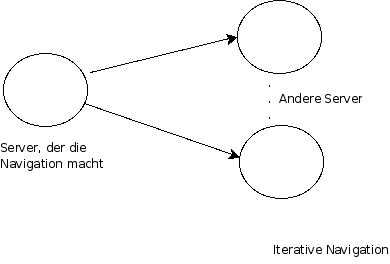
\includegraphics[width=90mm]{vsx06.png}
		\end{center}
		\end{figure}
	\item Rekursive Navigation
		\begin{itemize}
			\item Server, die nach Namen gefragt werden, kontaktieren ihrerseits aktiv weitere Server.
		\end{itemize}
\end{itemize}

\section{Verzeichnisdienste (Directory Service, Yellow Pages)}
Gesucht wird nach einer Dienstleistung. Es ist ``egal'', wer diesen Dienst anbietet. 
\begin{itemize}
	\item ``Drucke ein Dokument auf einem nahen Drucker''.
	\item ``Gib mir eine Wettervorhersage''
\end{itemize}
Verzeichnisdienst:
\begin{itemize}
	\item Gib mir alle (einen, mehrere) Namen mit den folgenden Attributen.
\end{itemize}

\chapter{\"{U}bungen}

\section{\"{U}bung 1}

\subsection{Aufgabe 1}

\subsubsection{Aufgabenstellung}
Geben Sie f\"{u}nf Typen f\"{u}r Hardware-Ressourcen und f\"{u}nf Typen f\"{u}r Daten-\\ oder Software-Ressourcen an, die sinnvoll gemeinsam genutzt werden k\"{o}nnen. Geben sie Beispiele f\"{u}r die gemeinsame Nutzung, wie sie in der Praxis in verteilten Systemen auftritt.

\subsubsection{L\"{o}sung}
Gemeinsam genutzte Ressourcen:
\begin{enumerate}
	\item Netzwerk (Hardware) 
		\begin{itemize}
			\item Gute Skalierbarkeit
			\item Relativ gute Positionstransparenz
			\item Gute Implementationstransparenz
		\end{itemize}
	\item Speicher (Arbeitsspeicher / RAM)
		\begin{itemize}
			\item Gemeinsame Nutzung durch Prozesse
		\end{itemize}
	\item Festplattenspeicher / Dateisystem
		\begin{itemize}
			\item Gut skalierbar
			\item Leicht benutzbar durch offene Schnittstelle (z.B. FTP, ...)
			\item Mitunter werden verschiedene Dateiformate verwendet!
		\end{itemize}
	\item Rechenleistung
		\begin{itemize}
			\item Seti-Projekt, leicht skalierbar 
			\item Wettervorhersage, schwer saklierbar im Sinne von VS
		\end{itemize}
	\item CAMPUS - HIS-QUIZ 
		\begin{itemize}
			\item Pr\"{u}fungsanmeldung
			\item Statuslisten
			\item Raumbelegungen
			\item Skalierbarkeit ist nicht so wichtig \textit{da die Anzahl der Studierenden sehr unwahrscheinlich sehr stark ansteigen wird}
			\item Hohe Sicherheitsanforderungen
		\end{itemize}
\end{enumerate}

\subsection{Aufgabe 2}

\subsubsection{Aufgabenstellung}
Wie k\"{o}nnen die Uhren in zwei Computern, die \"{u}ber ein lokales Netzwerk verbunden sind, ohne Benutzung einer externen Uhr synchronisiert werden? Welche Faktoren schr\"{a}nken die Genauigkeit ein? Welche Methoden zur Verbreitung der Zeit kennen Sie? Wie genau sind Sie?

\subsection{Aufgabe 3}

\subsubsection{Aufgabenstellung}
Die Kerntechnologien des WWW f\"{u}r die Anzeige von Informationen sind HTML, URLs und HTTP. Erl\"{a}utern Sie jeweils ihre Funktionen und welches Ziel durch ihren Einsatz erreicht wird. Sind die Technologien als allgemeine Grundlage von Client/Server-Programmierung ausreichend und geeignet?

\subsubsection{L\"{o}sung}
\begin{itemize}
	\item HTML (\textbf{H}yper\textbf{t}ext \textbf{M}arkup \textbf{L}anguage)
		\begin{itemize}
			\item Grammatik, Syntax, Semantik
			\item Standardisierung
			\item Offenheit
			\item Leichte Verwendbarkeit
			\item Implementationsunabh\"{a}ngigkeit
			\item Erweiterbarkeit
		\end{itemize}
	\item URL (\textbf{U}niform \textbf{R}esource \textbf{L}ocator)
		\begin{itemize}
			\item Bsp.: http://www.webmail.fh-aachen.de/ossmann/arbk/pra1.zip
				\begin{enumerate}
					\item Domain Name Servie: Macht aus dem Hostnamen eine IP-Nummer
					\item \textit{Anfrage des Servers auf den jew. Port}
					\item \textit{Anfrage des Servers auf das jew. Unterverzeichnis}
				\end{enumerate}
			\item Eindeutige Bezeichnung in verteilten Systemen
			\item Orts. bzw. Positionstransparenz
			\item Einigkeit \"{u}ber die Interpretation von Zeichen
			\item Bereitstellung eines Namensraums
		\end{itemize}
	\item HTTP (\textbf{H}yper\textbf{t}ext \textbf{T}ransfer \textbf{P}rotocol) 
		\begin{itemize}
			\item Offenheit
			\item Standardisierung
			\item Implementationsunabh\"{a}ngig
			\item HTTP ist \"{u}blicherweise nicht gut geeigent beliebige Client-Server Anwendungen zu realisieren
		\end{itemize}
\end{itemize}

\subsection{Aufgabe 4}

\subsubsection{Aufgabenstellung}
Geben Sie Beispiele von URLs an, und geben sie an, was die einzelnen Teile bedeuten. Inwiefern wird mit URLs das Ziel der Positionstransparenz erreicht? Wozu dient der DNS im Internet. Auch in Programmiersprachen werden Namen verwendet, wozu? Gibt es Parallellen zu URLs?
\subsubsection{L\"{o}sung}
\textit{``Bischen'' miterledigt in Aufgabe 3 meint der Prof.}

\subsection{Aufgabe 5}

\subsubsection{Aufgabenstellung}
Die Durchf\"{u}hrung einer Wahl in einem demokratischen Staat kann als Operation in einem verteiltem System aufgefasst werden. \"{U}blicherweise gibt es einen Wahlleiter, der die Wahl organisiert, durchf\"{u}hrt und Ergebnisse feststellt. Welche Arten von Fehlern werden normalerweise ber\"{u}cksichtigt (Fehlermodell)? Welche Arten von Angriffen (Sicherheitsmodell) werden normalerweise ber\"{u}cksichtigt? Versuchen Sie eine Interaktionsmodell zu erstellen, das die beteiligten Komponenten und ihre Beziehungen sichtbar macht.
\subsubsection{L\"{o}sung}
\begin{figure}[htbp]
\begin{center}
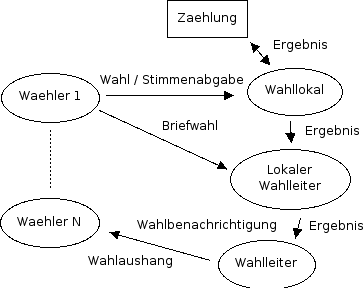
\includegraphics[width=100mm]{vsu3.png}
\end{center}
\end{figure}
Siehe Grafik.
\subsection{Aufgabe 6} 

\subsubsection{Aufgabenstellung}
Es soll ein Dienst ``INFO'' realisiert werden. INFO verwaltet eine potentiell sehr grosse Menge von Informationen als gemeinsam nutzbare Ressource, auf welche Benutzer durch Angabe eines Schl\"{u}ssels (Zeichenkette) zugreifen k\"{o}nnen. Diskutieren Sie, wie Sie die Namensgebung (d.h. Schl\"{u}sselbezeichnunge) organisieren, damit ein geringer Leistungsverlust entsteht, wenn die Anzahl der Ressourcen (Informationne), die verwaltet werden mu{\ss}, steigt. Schlagen Sie vor, wie Sie INFO implementieren, damit Leistungsengp\"{a}sse vermieden werden, wenn die Anzahl der Benutzer sehr gross ist.

\subsubsection{L\"{o}sung}
\textit{Bsp.: www.gpsies.com, Website die alle Routen f\"{u}r Rad-, Jogger- und Wanderwege. Ohne Bilder w\"{u}rde der Dienst weniger Speicher ben\"{o}tigen als mit Bilder. F\"{u}r die Streken m\"{u}ssen jedoch alle Wegpunkte vorhanden sein, da ein Weg nie ``nur'' geradeaus f\"{u}hrt. 1MB Text w\"{u}rde ca 80 Seiten Text entsprechen. Anzahl der Wegpunkte ist hier ca. auf 150 pro Weg beschr\"{a}nkt. Das w\"{a}ren dann ca. 8 Byte an Daten pro Wegstrecke. 32 Bit f\"{u}r eine Erdkoordinate entspricht eine Genauigkeit auf 10cm.}

\begin{itemize}
	\item Rundtouren haben Namen als Schl\"{u}ssel
	\item Jede Rundtour besteht aus $< 5000$ Wegpunkten a $20$ Bytes, d.h. $100$KBytes/Tour
	\item Derzeit $< 10000$ Touren f\"{u}r Deutschland 
	\item D.h. zur Zeit ca $1$GByte Speicher n\"{o}tig
	\item Wenn alle Betrachter von Touren nur 1 Server zur Verf\"{u}gung haben und die Anzahl der Betrachter w\"{a}chst, wird der Server zum Engpass!
		\begin{enumerate}
			\item Ausweg: Mehrere Server die den gesamten Datenbestand anbieten. (Ist aus Backup-Gr\"{u}nden sowieso gut!)
		\end{enumerate}
	\item Weiteres Wachstum der Betrachterzahl
	\item Wenn alle Server am gleichen Ort stehen wird das Netzwerk zum Engpass
		\begin{enumerate}
			\item Netzwerk besser machen
			\item Bringe die Daten n\"{a}her zum Benutzer durch Einrichten lokaler Server
		\end{enumerate}
	\item Erweiterung: Jede Tour kann mit Fotos und Videos erweitert werden. Jede Tour ben\"{o}tigt eventuell $20$ MByte.
		\begin{itemize}
			\item Idee: Jeder Server speichert nur die Touren, die ``in der N\"{a}he'' liegen.
			\item Vorsicht: Es w\"{a}re schlecht, wenn jede Tour nur auf einem Server gespeichert w\"{a}re. D.h. nun sollte die gesamte Information mehrfach verteilt speichern.
			\item Vorsicht: Es ist jetzt viel schwerer, eine konsistente Ansicht des Systems herzustellen
		\end{itemize}
	\item Eventuell vergeben Benutzer gleiche Namen f\"{u}r verschiedene Touren (z.B. ``Rund um den See'')
	\item Durch Erweiterung (z.B. Benutzername, Regionsname, L\"{a}ndername, Kontinentname, ...) kann man wieder eindeutige Namen herstellen
	\item Intern verwende eindeutige Nummerierung o.\"{A}.
\end{itemize}

\subsection{Aufgabe 7} 

\subsubsection{Aufgabenstellung}
In der Programmiersprache C benutzten Programme (Prozese) einfache sequentielle Dateien, die das Betriebssystem per FAT32 verwaltet. Welchen Service erbring das Dateisystem. Welche Operationsmenge wird realisiert? Wird Implementationstransparenz erreicht? Kann man die Benutzung als Client-Server Anwendung auffassen? Mu{\ss} ein Benutzer wissen, wo seine Daten auf der Festplatte stehen? K\"{o}nnen in diesem Beispiel Ressourcen von mehreren genutzt werden?

\subsubsection{L\"{o}sung}
Welche Dienstleistung erbringt ein Dateisystem? Welche Operationen werden durch Dateisystem erbracht?
\begin{enumerate}
	\item Verwaltung von ``Dateien'' die durch \underline{Dateinamen} bezeichnet werden
	\item Schreiboperationen
	\item Leseoperationen
	\item Open: Dateiname $\ra$ Dateihandle
	\item Close: Dateihandle
	\item Verzeichnisdienst (\textit{Macht aus einem Dateinamen eine Referenz})
	\item Gegen\"{u}ber einer Reihe von Varianten (z.B. Festplattengr\"{o}sse, FAT16, FAT32, Clusterung, Fragmentierung, ...) ist Implementationstransparenz erreicht
	\item Man kann nicht beliebig leicht zwischen Betriebssystem wechseln
	\item Bei USB-Datentr\"{a}gern hat man das Ziel der Implementationstransparenz st\"{a}rker ber\"{u}cksichtigt als bei Festplatten (\textit{daher wird bei den Sticks auch meistens ein FAT-Dateisystem verwendet, da dies relativ einfach aufgebaut ist und von den meisten Betriebssystemen gelesen werden kann}).
	\item Positonstransparenz ist erreicht. Der Benutzer mu{\ss} nichts \"{u}ber den physikalischen Ort der Dateien wissen.
	\item Grunds\"{a}tzlich ist vorgesehen, dass mehrere Prozesse die gleiche Datei nebenl\"{a}ufig benutzen.
\end{enumerate}

\subsection{Aufgabe 8} 

\subsubsection{Aufgabenstellung}
Ein Dienst wird von mehreren Servern implementiert. Geben sie Gr\"{u}nde daf\"{u}r an, warum es sinnvoll sein kann, Ressourcen zwischen den Servern zu \"{u}bertragen. Ist es zufriedenstellend, wenn Clients ihre Anfrage nach einem Dienst durch Multicast-Nachrichten stellen? L\"{a}sst sich so Mobilit\"{a}tstransparenz erreichen?

\subsubsection{L\"{o}sung}
Beispiel: Benutzer hat ``Web-Space''. Der Anbieter bringt diese Daten sinvollerweise auf einen Server der ``nahe'' beim Benutzer ist. Wenn der Benutzer sich bewegt (Wohnortwechsel AC $\ra$ NYC) sollten sich die Daten mitbewegen.\\
\\
Wenn man nicht weiss, wo eine Ressource liegt, k\"{o}nnte man eine Multicast-Nachricht an die Gruppe der m\"{o}glichen Orte nach der Ressource fragen.
\begin{itemize}
	\item Wenn alle Benutzer immer mit einem Multicast nach einer Ressource fragen erzeugt das sehr  viel unn\"{o}tigen Verkehr im Netz.
	\item Viele Server werden erfolglos gefragt
\end{itemize}
Richte einen Verzeichnis- oder Namensdienst ein.

\subsection{Aufgabe 9} 

\subsubsection{Aufgabenstellung}
Ein Server-Programm, das in einer bestimmten Programmiersprache erstellt wurde, stellt die Implementierung eines Objekts bereit, welches f\"{u}r den Zugriff durch Clients vorgesehen ist, die in anderen Programmiersprachen geschrieben wurden. Geben Sie Probleme an, die durch die Heterogenit\"{a}t verursacht werden. Wie kann man Sie l\"{o}sen?

\subsubsection{L\"{o}sung}
Grund-Datentypen: integer, char, byte, float, double, ... $\Ra$ Konvertierung zwischen den Sprachen mu{\ss} geregelt werden.
\begin{figure}[htbp]
\begin{center}
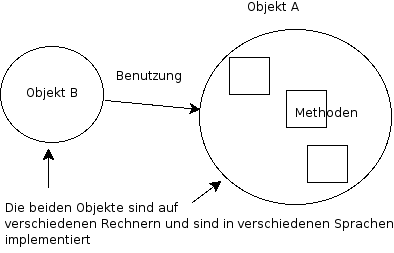
\includegraphics[width=90mm]{vsu4.png}
\end{center}
\end{figure}
\begin{itemize}
	\item Oft mu{\ss} Einigkeit \"{u}ber die Darstellung im Speicher erzielt werden (Little-Endian, ..., Zeichens\"{a}tze, ...).
	\item Es kann sein, dass eine Sprache, Maschine, usw. andere zusammengesetze Datentypen hat (array, struct, enum).
	\item Evtl. mu{\ss} man zusammengesetzte Datentypen nachbilden oder zwischen Typen konvertieren.
	\item Methodenaufruf: 
		\begin{enumerate}
			\item Parameter\"{u}bergabemechanismen
			\item Namensr\"{a}ume
			\item Wie werden Objektreferenzen dargestellt?
		\end{enumerate}
\end{itemize}


\section{\"{U}bung 2}

\subsection{Aufgabe 1}

\subsubsection{Aufgabenstellung}
Welche Faktoren beeinflussen die Antwortzeiten von Applikationen, die auf von einem Server verwaltete gemeinsam genutzte Daten zugreifen. Beschreiben Sie m\"{o}glichst L\"{o}sungsanst\"{a}tze um zu kleinen Antwortzeiten zu gelangen. Wie sinnvoll sind diese?

\subsubsection{L\"{o}sung}
Einflussfaktoren:
\begin{figure}[htbp]
\begin{center}
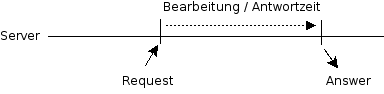
\includegraphics[width=95mm]{vsu5.png}
\end{center}
\end{figure}
\begin{itemize}
	\item Anzahl der User (Clients). \\
		\\
		$\Ra$ Durch Erh\"{o}hung der Anzahl der Server kann man versuchen die Zahl der Clients pro Server zu erniedrigen. Wenn zwischen den Servern nicht zu viel Koordination erforderlich ist, wird das die Antwortzeit erniedrigen.
	\item Werden im mittel mehrere Clients nebenl\"{a}ufig bedient, steigt f\"{u}r Jeden die Antworteit.
	\item Komplexit\"{a}t des Problems. Schwere Probleme erfordern lange Rechenzeit.\\
		\\
		$\Ra$ Bessere Algorithmen, bessere Implementation, bessere CPU, besserer Rechner.
	\item Andere Prozesse auf dem gleichen Rechner welche CPU-Zeit brauchen.\\
		\\
		$\Ra$ Verteilung der verschiedenen Dienste auf verschiedene Rechner bzw. CPUs.
	\item Schlechtes Scheduling, schlechte Performance des Betriebssystems\\
		\\
		$\Ra$ Betriebssystem anpassen, anders konfigurieren, anderes Betriebssystem.
\end{itemize}

\subsection{Aufgabe 2}

\subsubsection{Aufgabenstellung}
Geben Sie Beispiele f\"{u}r Fehler in Hardware und Software an, die durch den Aufbau von Redundanz vermieden werden k\"{o}nnen. Ist der Einsatz im Einzelnen sinnvoll?

\subsubsection{L\"{o}sung}
Hardware:
\begin{itemize}
	\item Netzteil f\"{a}llt aus\\
		\\
		$\Ra$ Mehrfache Netzteile, ist technisch aufw\"{a}ndig, geht aber. Ist f\"{u}r normale Benutzer (PC-Bereich) zu teuer aber f\"{u}r hochverf\"{u}gbare Anwendungen realisiert.
	\item Festplatten-Crash\\
		\\
		$\Ra$ RAID-Systeme a.\"{A}. sch\"{u}tzen vor dem Einzelausfall. Man mu{\ss} eigentlich pr\"{u}fen, ob durch das Hinzuf\"{u}gen wirklich die Ausfallrate sinkt!
\end{itemize}
Software:
\begin{itemize}
	\item Benutze ``Exceptions'' um Fehler abzunfangen, die ihre Software selbst feststellt. Der Programmierer bringt alle Exceptions die ihm bekannt sind! 
		\begin{itemize}
			\item Eventuell f\"{u}hren nicht ber\"{u}cksichtigte Exceptions zum Prozessabbruch.
			\item Kann eventuell abgefangen und durch Redundanz maskiert werden (\textit{z.B. gleiches Programm auf anderem Betriebssystem und/oder in einer anderen Programmiersprache})
		\end{itemize}
	\item Fehlerhafter Algorithmus
		\begin{itemize}
			\item Doppelte Implementation bringt da nichts.
			\item Eventuell kann man leicht feststellen, dass ein Ergebnis fehlerhaft ist (z.B. beim Sortieren).
			\item Verschiedene Algorithmen + verschiedene Implementationen + verschiedene Betriebssysteme + ..., k\"{o}nnten helfen. Aber das ist extrem aufw\"{a}ndig.
		\end{itemize}
\end{itemize}

\subsection{Aufgabe 3}

\subsubsection{Aufgabenstellung}
Betrachten Sie einen einfachen Server, der Client-Anforderungen ausf\"{u}hrt, ohne auf anderen Server zuzugreifen. Erkl\"{a}ren Sie, warum es im Allgemeinen nicht m\"{o}glich ist, eine Begrenzung f\"{u}r die Zeit zu setzen, die es dauern darf, bis ein solcher Server auf eine Client-Anforderung reagiert. Was w\"{a}re erforderlich, damit der Server Anforderungen in einer begrenzten Zeit ausf\"{u}hren kann? Ist dies eine praktikable Option?

\subsubsection{L\"{o}sung}
\begin{itemize}
	\item Scheduling ist unvorhersagbar
	\item Seitenfehler oder allgemein Verf\"{u}gbarkeit von Ressourcen ist schwer vorhersagbar
	\item Netzwerkaspekte sind schwer vorhersagbar
	\item Caching-Effekte
\end{itemize}
Im Normalfall kann man diese Effekte nicht so gut kontrollieren, dass man Garantien abgeben kann. Viele Effekte kann der Anwendungsprogrammierer selbst nicht beeinflussen.

\subsection{Aufgabe 4}

\subsubsection{Aufgabenstellung}
Geben Sie f\"{u}r jeden der Faktoren, die zu der Zeit beitragen, die es dauern, eine Nachricht zwischen zwei Prozessen \"{u}ber einen Kommunikationskanal zu \"{u}bertragen, an, welche Massnahmen erforderlich sind, um einen Grenzwert f\"{u}r seinen Beitrag zur Gesamtzeit vorzugeben. Warum werden diese Massnahmen in den aktuellen allgemeinen verteilten Systemen nicht angewendet?

\subsubsection{L\"{o}sung}

\textit{Haben wir schon genug zu gesagt meint der Prof}

\subsection{Aufgabe 5}

\subsubsection{Aufgabenstellung}
Angenommen, ein grundlegender Lesevorgang von einer Festplatte liest manchmal Werte, die sich von den geschriebenen unterscheiden. Schlagen Sie vor, wie dieser Fehlertyp erkannt bzw. maskiert werden kann um einen weniger schwerwiegenden Fehlertyp zu erzeugen.

\subsubsection{L\"{o}sung}

\begin{enumerate}
	\item Idee: Speichere zus\"{a}tzliche Pr\"{u}finformationen (Parit\"{a}tsbits, Pr\"{u}fsummen, ...)
	\item Idee: Mehrfaches Lesen $\Ra$ Mehrheitsentscheid
		\begin{itemize}
			\item Lese 10 mal hintereinander
			\item Restfehlerwahrscheinlichkeit ganz grob $(P_E)^N$ mit $P_E := $ Einzelfehler. \textit{F\"{u}r keine Restfehlerwahrscheinlichkeit: $n \ra $ unendlich}.
			\item W\"{a}hle $N$ so, dass die Fehlerrate ausreichend niedrig ist, d.h. dass z.B. andere Fehler h\"{a}ufiger oder schwerwiegender sind.
			\item Falls (z.B. bei kleinem $N$) kein vern\"{u}nftiger Mehrheitsentscheid m\"{o}glich ist, sollte man dem Benutzer den Fehler mitteilen.
		\end{itemize}

\end{enumerate}

\subsection{Aufgabe 6}

\subsubsection{Aufgabenstellung}
Ein Client versucht, eine Synchronisierung mit einem Zeit-Server durchzuf\"{u}hren. Er zeichnet in der nachfolgend gezeigten Tabelle die Round-Tip-Zeiten und die Zeitstempel auf, die vom Server zur\"{u}ckgegebe wurden.\\
\\
\begin{tabular}{c|c}
	\textbf{Round-Trip (ms)} & \textbf{Zeitstempel (h:min:sec)} \\
	\hline 
	22 & 10:54:23.674 \\
	25 & 10:54:25.450 \\
	20 & 10:54:28.342 
\end{tabular}
\\
\\
Welche dieser Zeiten sollte er verwenden um seine Uhr zu setzen. Auf welche Zeit sollte er sie setzen? Sch\"{a}tzen Sie die Genauigkeit der Einstellung. \"{A}ndern sich die Antworten, wenn bekannt ist, dass die Zeit zwischen Senden und Empfangen einer Nachricht im System mindestens 8ms betr\"{a}gt?

\subsubsection{L\"{o}sung}
\begin{figure}[htbp]
\begin{center}
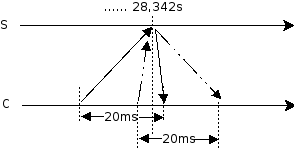
\includegraphics[width=80mm]{vsu6.png}
\end{center}
\end{figure}
Nehme die kleinste Round-Trip-Zeit weil damit die Ungenauigkeit minimal wird. (Bild). Empfangene Zeitstempel: $\frac{RTT}{2} = 10$ms.  D.h. hier setzt der Client seine Zeit auf $28,342$ms $+10$ms $= 28,352$s. Genauigkeit kann um $10$ms abweichen.\\
\\
Wenn zus\"{a}tzlich bekannt ist, dass eine Nachricht mindestens $8$ms braucht, nimmt man nach wie vor zur Synchronisation das Paar mit der kleinsten Round-Trip Zeit.\\
\\
Diagramm mit den Extremf\"{a}llen bei $20$ms RTT und mindestens $8$ms Nachrichtenverz\"{o}gerung.
\begin{figure}[htbp]
\begin{center}
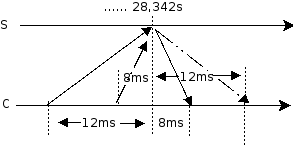
\includegraphics[width=80mm]{vsu7.png}
\end{center}
\end{figure}
Setze eigene Uhr auf $28,342s + \frac{20ms}{2}= 28,352s$\\
\\
Jetzt ist die Garantiegenauigkeit $\pm 2ms$\\
\\
$2ms = \frac{1}{2} (20ms - 2*8ms)$
\subsection{Aufgabe 7}
\subsubsection{Aufgabenstellung}
Im folgenden Diagramm ist f\"{u}r 4 Prozesse die zeitliche Abfolge von Ereginissen und Nachrichten (Senden/Empfangen) angegeben. Ordnen Sie den Ereignissen Lamport-Zeitstempel zu. Gibt es nebenl\"{a}ufige Ereignisse? (Bild).

\subsubsection{L\"{o}sung}
Alle Ereignisse von $P_1$ und $P_2$ sind nebenl\"{a}ufig zu allen Ereignissen aus $P_3$ und $P_4$ weil zwischen diesen Paaren keine Kommunikation stattfindet.
\begin{figure}[htbp]
\begin{center}
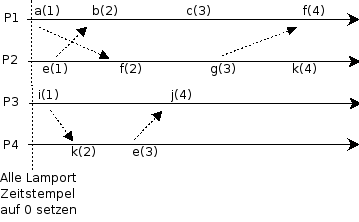
\includegraphics[width=80mm]{vsu8.png}
\end{center}
\end{figure}
Ereignise die den gleichen Lamport-Zeitstempel haben sind nebenl\"{a}ufig.

\subsection{Aufgabe 8}

\subsubsection{Aufgabenstellung}
Zur Zuordnung von Zeistempeln sollen nun Vektoruhren verwenden werden. Ordnen Sie den Ereignissen aus Aufg. 7 Vektor-Zeitstempel zu.

\subsubsection{L\"{o}sung}
Siehe Grafik.
\begin{figure}[htbp]
\begin{center}
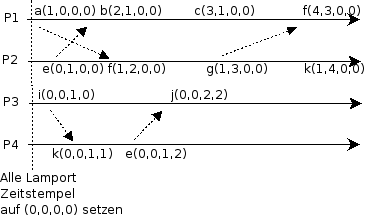
\includegraphics[width=80mm]{vsu9.png}
\end{center}
\end{figure}

\section{\"{U}bung 3}
\subsection{Aufgabe 1}

\subsubsection{Aufgabenstellung}
Gegeben ist der folgende Ablauf von zwei Prozessen $P_1$ und $P_2$ mit insgesamt 5 Ereignissen. Aufgrund von Vektorzeitstempeln k\"{o}nnen Sie die globale Relation $\ra$ zwischen Ereignissen auswerten. Sie verf\"{u}gen aber nicht \"{u}ber die Kenntnis der zeitlichen Reihenfolge von Ereignissen.

\begin{figure}[htbp]
\begin{center}
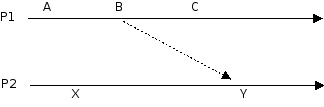
\includegraphics[width=70mm]{vsu3a1.png}
\end{center}
\end{figure}

\begin{enumerate}
	\item Geben Sie die Historien history($P_1$) und history($P_2$) an!
	\item Geben Sie einen RUN des Systems an der keine LINEARISIERUNG des Systems ist! Geben Sie einen konsistenten und einen inkonsistenten Schnitt des Systems an. Geben Sie die Linearisierung an, die durch die zeitliche Reihenfolge festgelegt ist! Skizzieren Sie die zugeh\"{o}rigen Schnitte!
	\item Geben Sie alle Linearisierungen des Systems an! Zeichnen Sie zu den Linearisierungen jeweils zugeh\"{o}rige zeitliche Abl\"{a}ufe in einem Diagramm \"{a}hnlich dem oben angegebenen!
\end{enumerate}


\subsubsection{L\"{o}sung}

\begin{enumerate}
	\item History ($P_1$) = $A B C$\\
		History ($P_1$) = $X Y$
	\item $CBAYX$ ist kein RUN und keine Linearisierung.\\
		\\
		$AXBCY$ ist ein RUN \textit{Weil $ABC$ ist in der richtigen Reihenfolge und auch $XY$ ist in der richtigen Reihenfolge}.\\
		\\
		$XYABC$ ist ein RUN aber keine Linearisierung, weil (z.B.) gegen $B \ra Y$ verstossen wird.
		\begin{figure}[htbp]
		\begin{center}
		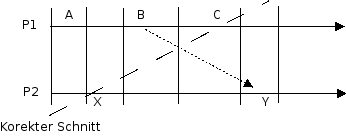
\includegraphics[width=70mm]{vsu3a1b.png}
		\end{center}
		\end{figure}

	\item Liste aller Linearisierungen\\
		\\
		$ABXZY$\\ 
		$ABXCY$\\ 
		$ABXYC$\\ 
		$AXBCY$\\ 
		$AXBYC$\\ 
		$XABCY$\\ 
		$XABYC$
\end{enumerate}


\subsection{Aufgabe 2}

\subsubsection{Aufgabenstellung}

In dieser Aufgab wird ein verteiltes System betrachtet, welches aus zwei Prozessen $P_1$ und $P_2$ besteht. Beide Prozesse verwenden eine Kopie der Datei $x$. Jede einzelne Kopie hat einen Zeitstempel. Die Kopie von Prozess $P_1$ hat Zeitstempel $a$, die Kopie von $P_2$ hat Zeitstempel $b$. Immer wenn ein Prozess an der Datei \"{A}nderungen (z.B. mit dem Editor) vornimmt, wird der Zeitstempel um 1 erh\"{o}t.\\
\\
Ein Prozess kann einem anderen die Datei inklusive Zeitstempel in einer Nachricht senden. Dann hat nach dem Empfang die Kopie des Empf\"{a}ngers den Zeitstempel der Kopie des Absenders.\\
\\
Am Anfang haben die beiden Prozesse die gleiche Version der Datei und beide Kopien haben den Zeistempel $a = b = 4710$.\\
\\
Die Systemadministrator hat die folgende Regel aufgestellt: Benutzer $P_2$ darf die Datei selbst nicht \"{a}ndern. Er darf immer nur Kopien benutzen, die er von $P_1$ erhalten hat. Es ist aber nicht klar, ob Benutzer $P_2$ sich immer an diese Regel h\"{a}lt.

\begin{enumerate}
	\item Man \"{u}berlege sich, dass, wenn die Regel eingehalten wird, der Zeitstempel $b$ nie gr\"{o}sser sein kann, als der Zeitstempel $a$. Ein interessantes Pr\"{a}dikat in diesem System ist also das Pr\"{a}dikat $b > a$.
	\item Der folgende Ablauf hat stattgefunden. Dabei bezeichnen $E$ das Editieren der lokalen Dateikopie, $S$ das Senden der lokalen Dateikopie und $R$ das Empfangen der lokalen Dateikopie. Man gebe jeweils die Zeitstempel an, die die Dateikopien erhalten!
	\item
		\begin{enumerate}
			\item Gibt es einen Zeitpunkt, zu dem $b > a$ wahr ist?
			\item Gilt ``m\"{o}glicherweise $b > a$?
			\item Gilt ``definitiv $b > a$?
		\end{enumerate}
		Sch\"{o}pft also der Systemadministrator in den vorliegenden Situationen Verdacht? Kann er anhand seiner Kenntnisse beweisen, dass $P_2$ unerlauberweise die Datei ge\"{a}ndert hat?
	\item Wie sieht ein Verlauf aus, in welchem ``m\"{o}glicherweise $b > a$'' nicht gilt? Sie d\"{u}rfen z.B. zus\"{a}tzliche Nachrichten versenden.
	\item Wie sieht ein Verlauf aus, in welchem ``definitiv $b > a$'' gilt, also ein Ablauf in welchem der Systemadministrator den Nachweis des Verstosses gegen die Regel erbringen kann. Sie d\"{u}rfen z.B. zus\"{a}tzliche Nachrichten einzeichnen.
\end{enumerate}

\subsubsection{L\"{o}sung}
\begin{enumerate}
	\item Wird $P_2$ nur durch Empfang neuer Versionen von $P_1$ den Wert von $b$ erh\"{o}t, kann nie $b > a$ sein (sofern sich $P_2$ an die Regeln h\"{a}lt).
			\begin{figure}[htbp]
			\begin{center}
			\includegraphics[width=90mm]{vsu3a2.png}
			\end{center}
			\end{figure}
	\item
			\textit{Was ist jedoch wenn $P_2$ sich nicht an die Regeln h\"{a}lt? Kann man das feststellen?}
			\begin{figure}[htbp]
			\begin{center}
			\includegraphics[width=90mm]{vsu3a2b.png}
			\end{center}
			\end{figure}
			Auswertung der ``$\ra$''-Relation kann der Systemadministrator mit Vektorzeitstempeln durchf\"{u}hren.\\
	\item 
		\begin{enumerate}
			\item Nach $E_3$ und vor $E_2$ ist $a = 4711$ und $b = 4712$
			\item ``m\"{o}glicherweise ist $b > a$'\\
				\\
				Im folgender Linearisierung\\
				\\
				$E_1 S_1 R_1 E_3 | E_2$\\
				\\
				gibt es einen globalen Zustand (der mit dem angedeuteten Schnitt aassoziert ist) in welchem $a = 4711\quad b = 4712$ ist, d.h. $b > a$. Es ist also m\"{o}glicherweise $b > a$.
			\item \textit{Frage anders ausgedr\"{u}ckt:} Gibt es in \underline{jeder} Linearisierung einen globalen Zustand (d.h. Schnitt) in welchen $b > a$?\\
				\\
				Um zu zeigen, dass (definitiv...) nicht gilt, reicht es also, eine Linearisierung zu finden bei welcher in keinem Zustand $b > a$ ist.\\
				\\
				\begin{tabular}{|l|l|l|l|l|l|}
					~ & $E_1$ & $S_1$ & $R_1$ & $E_2$ & $E_3$ \\
					$a=4710$ & $4711$ & $4711$ & $4711$ & $4712$ & $4712$\\
					$b=4710$ & $4710$ & $4710$ & $4711$ & $4711$ & $4712$
				\end{tabular}
		\end{enumerate}
\end{enumerate}

\subsection{Aufgabe 3}

\subsubsection{Aufgabenstellung}
In einem verteilten System wollen zwei Prozesse hintereinander auf einen gemeinsamen Drucker drucken. Durch einen ``Token'' soll der Zugriff geregelt werden. Nur der Prozess, der das ``Token'' hat, darf drucken. Ein Prozess darf durch Nachrichten an den anderen Prozess versuchen, das Token zu bekommen. Er erh\"{a}lt das Token ebenfalls durch Nachrichtenversand. Veranschaulichen Sie sich, welche Arten von Abl\"{a}ufen mit Ereignissen sich prinzipiell ergeben. Wie kann man erreichen, dass\\
\\
$~ \quad $ m\"{o}glicherweise(``$P_1$ druckt'' und ``$P_2$ druckt'')\\
\\
nicht wahr ist! Gehen sie davon aus, dass Nachrichten fehlerfrei gesendet und empfangen werden.

\subsubsection{L\"{o}sung}
Ereignisse: $A$ Anfang des Druckens, $E$ Ende des Druckens. 
\begin{figure}[htbp]
\begin{center}
\includegraphics[width=100mm]{vsu3a3.png}
\end{center}
\end{figure}
Man m\"{o}chte nicht, dass sich Druckerbelegungen \"{u}berlappen. D.h. man will wechselseitigen Ausschluss.\\
\\
Wenn zwei Prozesse in einem globalen Zustand (d.h. konsistenten Schnitt) jeweils $A$ gemacht haben, und noch keiner $E$, dann sei das Pr\"{a}dikat ``Konflikt'' wahr.
\begin{figure}[htbp]
\begin{center}
\includegraphics[width=100mm]{vsu3a3b.png}
\end{center}
\end{figure}
In einem so programmierten System ist das Pr\"{a}dikat definitiv ($\overline{Konfkikt}$) wahr. Denn in jeder Linearisierung gibt es den angedeuteten Zustand $A_1 | ...$ in welchem $\overline{Konflikt}$ wahr ist.\\
\\
Deswegen ist das Pr\"{a}dikat ``definitiv ($\overline{Konflikt}$)'' f\"{u}r diese Aufgabenstellung nicht hilfreich.\\
\\
Das Pr\"{a}dikat m\"{o}glicherweise (Konflikt) ist besser. Wenn m\"{o}glicherweise (Konflikt) unwahr ist, hei{\ss}t das, dass es in keiner Linearisierung irgendeinen globalen Zustand gibt, in welchem ein Konfliktkt besteht. Das ist das, was man will.\\
\\
Man regele Zugriff durch ein Token. Ein Prozess darf $A$ nur ausf\"{u}hren , wenn er das Token besitzt. Solange ein Prozess ``zwischen $A$ und $E$ ist, darf er das Token nicht versenden. Wir gehen $P_1$ am Anfang des Tokens. Durch die Regeln ist jetzt die Konfliktfreiheit sichergestellt.

\subsection{Aufgabe 4}
\subsubsection{Aufgabenstellung}
Es sei $\varphi$ ein Pr\"{a}dikat in einem verteilten System. Beweisen Sie, dass aus definitiv (nicht $\varphi$) nicht folgt nicht (m\"{o}glicherweise($\varphi$)).

\subsubsection{L\"{o}sung}
Zu zeigen ist: Aus definitiv($\overline{\varphi}$) folgt nicht $\overline{moeglicherweise \quad \varphi}$.\\
\\
Es reicht, ein Beispiel bei welchen definitiv $\overline{\varphi}$ gilt und m\"{o}glicherweise $\varphi$.

\begin{itemize}
	\item definitiv $\overline{\varphi}$: In jeder Linearisierung gibt es jeweils einen globalen Zustand, so dass $\varphi$ unwahr ist.
	\item m\"{o}glicherweise $\varphi$: Es gibt eine Linearisierung, so dass $\varphi$ wahr ist.
\end{itemize}
Pr\"{a}dikate werden in globalen Zust\"{a}nden (Schritten) ausgewertet. Ihr Wahrheitswert kann sich \"{a}ndern.\\
\\
Betrachte Zuweisungen an Variable als Ereignisse. 
\begin{figure}[htbp]
\begin{center}
\includegraphics[width=60mm]{vsu3a4.png}
\end{center}
\end{figure}
Im Schnitt $S$ hat $x$ den Wert 5, d.h. $x == 5$ ist ``true''.
\begin{figure}[htbp]
\begin{center}
\includegraphics[width=60mm]{vsu3a4b.png}
\end{center}
\end{figure}
Pr\"{a}dikat $\varphi$: $x = 1$. Im zweiten Bild wird gezeigt:\\
\\
$S_1$ zeigt, dass 1 gilt\\
$S_2$ zeigt, dass 2 gilt

\section{\"{U}bung 4}

\subsection{Aufgabe 1}

\subsubsection{Aufgabenstellung}
Der Algorithmus von Maekawa zum wechselseitigen Ausschluss soll f\"{u}r $N=16$ Prozesse implementiert werden. Es soll die in der Vorlesung behandelte einfache Methode zur Bestimmung der W\"{a}hlermengen angewandt werden. Die Prozesse seien von $1..16$ durchnummeriert.
\begin{enumerate}
	\item Geben Sie f\"{u}r die Prozesse $1, 2, 5, 6, 8$ die W\"{a}hlermengen an!
	\item In wievielen W\"{a}hlermengen ist ein Prozess jeweils enthalten?
	\item Eine Fordernung an die W\"{a}hlermengen ist, dass je zwei W\"{a}hlermengen mindestens ein gemeinsames Element haben m\"{u}ssen. Ist diese Forderung auch erf\"{u}llt, wenn man die W\"{a}hlermengenbestimming z.B. f\"{u}r $N=12=3*4$ mit einer rechteckigen $3*4$ Matrix anstelle mit einer quadratischen Matrix durchf\"{u}hrt. Kann man stattdessen auch eine $1$x$12$ Matrix nehmen?
\end{enumerate}


\subsubsection{L\"{o}sung}

\begin{tabular}{cccc}
1 & 2 & 3 & 4 \\
5 & 6 & 7 & 8 \\
9 & 10 & 11 & 12 \\
13 & 14 & 15 & 16 
\end{tabular}
\\
\\
$V_1 = \{1, 2, 3, 4, 5, 9, 13\}$\\
$V_2 = \{1, 2, 3, 4, 6, 10, 14\}$\\
$V_5 = \{1, 5, 6, 7, 8, 9, 13\}$\\
$V_6 = \{2, 4, 5, 7, 8, 10, 14\}$\\
$V_8 = \{4, 5, 6, 7, 8, 12, 16\}$\\
\\
Jede W\"{a}hlermenge hat $7 = 2*4-1 = 2*\sqrt{16} - 1 = 2 * \sqrt{N} - 1$ Elemente.\\
\\
Jeder Teilnehmer ist in $7 =  \sqrt{N} - 1$ Mengen enthalten.\\
\\
\begin{tabular}{cccc}
1 & 2 & 3 & 4 \\
5 & 6 & 7 & 8 \\
9 & 10 & 11 & 12 
\end{tabular}
\\
\\
$V_1 = \{2, 5, 6, 7, 8, 10\}$\\
\\
\textit{Man darf es auch mit einer rechteckigen Matrix machen: Jeder kommt gleichviel in jeder W\"{a}hlermenge vor.}\\
\\
\begin{tabular}{cccccccccccc}
1 & 2 & 3 & 4 & 5 & 6 & 7 & 8 & 9 & 10 & 11 & 12 
\end{tabular}
\\
\\
$V_1 = \{1, 2, .., 12\}$\\
\\
\textit{Man darf es auch mit einer extrem rechteckigen Matrix machen. Jeder kommt gleichviel in jeder W\"{a}hlermenge vor.}\\
\\
Erweiterung: Was macht man f\"{u}r $N = 13$\\
\\
\begin{tabular}{cccc}
1 & 2 & 3 & 4 \\
5 & 6 & 7 & 8 \\
9 & 10 & 11 & 12 \\
13 & & & 
\end{tabular}
\\
\\
Wenn man nun die ``Zeilen-Spalten''-Konstruktion macht, ist die Frage, ob man noch W\"{a}hlermengen erh\"{a}lt, die wechselseitigen Ausschluss sichern. \\
\\
$V_1 = \{1, 2, 3, 4, 5, 9, 13\}$ hat 7 Elemente\\
$V_2 = \{1, 2, 3, 4, 6, 10\}$ hat 6 Elemente\\
$V_{13} = \{1, 6, 9, 13\}$ hat 4 Elemente\\
\\
Die W\"{a}hlermengen sind nicht mehr alle gleich gross und Teilnehmer sind verschieden oft in W\"{a}hlermengen enthalten.\\
\\
Durch Eintragen ``von oben'' ist gesichert, dass 1 gemeinsames Element bleibt.\\
\\
Wenn ein Teilnehmer abst\"{u}rzt, mu{\ss} man neue W\"{a}hlermengen bestimmen. Frage: Darf man den abgest\"{u}rzten Teilnehmer einfach aus allen W\"{a}hlermengen rausnehmen?\\
\\
\begin{tabular}{cccc}
1 & 2 & 3 & 4 \\
5 & 6 & 7 & 8 \\
9 & 10 & 11 & 12 \\
13 & & & 
\end{tabular}
\\
\\
\textit{Wenn man Teilnehmer 13 rausnehmen w\"{u}rde, dann g\"{a}be es kein Problem.} Falls 5 abst\"{u}rzt und entfernt wird, ist $V_7 = \{3,\not{5}, 6, 7, 8, 11\}$ und $V_{13} = \{1,\not{5}, 9, 13 \}$. D.h. $V_7$ und $V_{13}$ haben kein gemeinsames Element mehr. Die Vorgehensweise, abgest\"{u}rzte Teilnehmer in allen W\"{a}hlermengen zu streichen ist unzul\"{a}ssig. 

\subsection{Aufgabe 2}

\subsubsection{Aufgabenstellung}
Das Durchf\"{u}hren einer Zentral-Abiturpr\"{u}fung kann als Operation in einem verteitel System betrachtet werden, wobei die Aufgaben per MULTICAST in die Teilnehmer versandt werden.
\begin{enumerate}
	\item Unterscheidet man bei diesem Problem zwischen ``Empfang'' und ``Auslieferung'' der Nachrichten?  Wann wird ausgeliefert?
	\item Wie wird bei dieser Aufgabe das Problem gel\"{o}st, dass dadurch entsteht, dass es in einem verteilten System keine globale Zeit gibt?
	\item Liegt einer solchen Prf\"{u}fungsopteration eher ein ``synchrones'' oder ein ``asynchrones'' Systemmodell zugrunde? Wie wird mit ''Nachrichtenverlust'' umgegangen?
	\item Finden Sie andere Beispiele daf\"{u}r, dass zwischen ``Empfang'' und ``Auslieferung'' einer Nachricht unterschieden wird!
\end{enumerate}

\subsubsection{L\"{o}sung}
\begin{enumerate}
	\item Die Aufgaben werden per Multicast an die Teilnehmer der Pr\"{u}fung verteilt. Im Normalfall treffen die Aufgaben ``beim Lehrer'' ein, werden aber an die Teilnehmer noch nicht ausgeliefert. Lehrer ist stellvertretend f\"{u}r die Middleware.
	\item Man verhindert die Kommunikation der Teilnehmer von dem Zeitpunkt an, bei dem die erste Aufgabe ausgeliefert wird. Weil es keine globale Zeit gibt, stoppt man die Kommunikation schon etwas vorher. Dabei setzt man implizit voraus, dass das System synchron ist. Die Aufgaben werden in der Realit\"{a}t einen gewissen Zeitraum vor der Auslieferung versandt um sicherzustellen, dass sie rechtzeitig da sind. Darauf kann man sich nur in einem synchronen System verlassen. Man will, dass entweder alle die gleichen Aufgaben l\"{o}sen, oder keiner irgendeine.
	\item Beim Design gehen alle davon aus, dass das System sich synchron verh\"{a}lt. Im Normalfall verh\"{a}lt sich die Realit\"{a}t f\"{u}r ein Zentralabitur auch ``synchron genug''.
\end{enumerate}
\subsection{Aufgabe 3}

\subsubsection{Aufgabenstellung}
In der Vorlesung wurde ein Algorithmus zum zuverl\"{a}ssigem Multicast vorgestellt.
\begin{enumerate}
	\item Wieviele Nachrichten werden dabei \"{u}ber 1:1 Kan\"{a}le versandt, wenn $N$ Prozesse teilnehmen und keine Prozesse abst\"{u}rzen? Ist die Anzahl davon abh\"{a}ngig, in welcher Reihenfolge Nachrichten bei Prozessen eintreffen?
	\item Sie modifizieren den Algorithmus dergestalt, dass ein Prozess nur noch an die Prozesse multicastet, von welchen er selbst noch keine Nachricht erhalten hat. \"{U}berlegen Sie sich f\"{u}r den Fall $N=4$ wie solch ein Ablauf dann aussehen kann. Kann man sagen, mit wievielen nachrichten man in deinem g\"{u}nstigen Fall auskommt?
\end{enumerate}


\subsubsection{L\"{o}sung}
\begin{enumerate}
	\item Jeder Prozess (Teilnehmer) schickt irgendwann im Rahmen seines Basic-Multicasts an jeden Teilnehmer eine Nachricht. D.h. insgesamt werden bei $N$ Teilnehmern $N^2$ Nachrichten verschickt.
	\item Im Schlimmsten Fall senden alle Teilnehmer nach dem Empfang der ersten Nachricht so schnell, dass sie keine weitere Nachricht empfangen, bevor sie mit dem Senden fertig sind. Dann $N + (N-1)^2$ Nachrichten.
		\begin{figure}[htbp]
		\begin{center}
		\includegraphics[width=65mm]{vsu4a2.png}
		\end{center}
		\end{figure}
		\begin{figure}[htbp]
		\begin{center}
		\includegraphics[width=85mm]{vsu4a2b.png}
		\end{center}
		\end{figure}
		Im optimalen Fall sind vermutlich $1 + 2 + 3 + ... + N = N + (N-1) + ... + 1$ Nachrichten erforderlich $= \frac{N * (N+1)}{2} \approx \frac{N^2}{2}$. Ist die gleiche Gr\"{o}ssenordnung aber immerhin Reduktion um $\frac{1}{2}$.	
\end{enumerate}

\subsection{Aufgabe 4}

\subsubsection{Aufgabenstellung}
Die ``ELECTION'' Schnittstelle stellt zwei entfernte Methoden bereit:
\begin{itemize}
	\item VOTE: Diese Methode verarbeitet zwei Parameter, mit denen ein Client den Namen eines Kandidaten (String) und die Nummer eines W\"{a}hlers (32-Bit Integer) \"{u}bergibt.
	\item RESULT: Diese Methode verarbeitet zwei Parameter, \"{u}ber die der Server dem Client den Namen des Kandidaten und die Anzahl der Stimmen f\"{u}r diesen Kandidaten mitteilt.
\end{itemize}
Welche Parameter dieser Methoden sind jeweils Eingabe-, welche Ausgabe-Parameter? Erkl\"{a}ren Sie Marshalling und Un-Marshalling an diesen Parametern.

\subsubsection{L\"{o}sung}

\begin{itemize}
	\item \texttt{VOTE} wird beim W\"{a}hlen aufgerufen
	\item \texttt{RESULT} wird nach der Wahl aufgerufen
\end{itemize}

\texttt{VOTE(name: STRING; Vnumber: int32)} Beides sind ``in-Parameter''.\\
\\
Darstellung in einer Nachricht
\begin{itemize}
	\item Methoden-ID: int32, Big-Endian 4 Bytes
	\item \texttt{STRING}: 
		\begin{enumerate}
			\item Variante: L\"{a}nge 1 Byte gefolgt von 16-Bit Zeichen, und zwar so viele, wie die L\"{a}nge angibt.
			\item Variante: Folge von Zeichen (z.B. Unicode) gefolgt von einem Terminierungszeichen.
		\end{enumerate}
		\begin{figure}[htbp]
		\begin{center}
		\includegraphics[width=80mm]{vsu4a4.png}
		\end{center}
		\end{figure}
\end{itemize}
Eventuell baut man ``R\"{u}ckabeparameter'' ein, um aufgetretene Fehler identifizieren zu k\"{o}nnen. Der Proxy k\"{o}nnte evtl. liefern:
\begin{itemize}
	\item ~0: Ich habe eine positive Antwort vom Election-Interface bekommen
	\item -1: Time-Out, keine Antwort in vorgegebener Zeit
	\item ...
\end{itemize}
Das w\"{a}re als ``out-Parameter'' zu betrachten und in der IDL so anzugeben.\\
\\
RESULT: Man gibt einen Kandidatennamen an und erh\"{a}lt wieviele Stimmen er in der Wahl erhalten hat.\\
\\
\texttt{RESULT(in Cname: STRING; out Cvotes: int32)}\\
\\
Marshalling wie oben. Eventuell zus\"{a}tzlich: Detektierte Fehler weiterreichen.

\subsection{Aufgabe 5}

\subsubsection{Aufgabenstellung}
Der ELECTION Dienst mu{\ss} sicherstellen, dass eine Wahl aufgezeichnet wird, wenn ein W\"{a}hler annimmt, dass er seine Wahl abgegeben hat. Beschreiben Sie, welche Auswirkung eine Vielleicht-Aufrufsemantik auf den ELECTION-Dienst hat. Ist eine Mindestens-Einmal Semantik f\"{u}r den ELECTION-Dienst ausreichend oder ist eine H\"{o}chstens-Einmal Semantik empfohlen.

\subsubsection{L\"{o}sung}
Bei einer ``Vielleicht'' Aufruf Semantik werden Stimmen, deren Nachrichten verloren gehen, nicht gez\"{a}hlt. Da nicht auf Antworten gewartet wird, wird auch nicht wiederholt. Da Nachrichtenverlust (z.B. bei UDP-Paketen) vorkommt, ist diese Korektheitsforderung zu schwach.\\
\\
Variante: Mindestens einmal:
\begin{itemize}
	\item Es werden so lange \texttt{VOTE}-Nachrichten geschickt, bis eine Antwort antrifft.
\end{itemize}
Bei dieser Variante filtert der Empf\"{a}nger mehrfach eintreffende \texttt{VOTE}-Aufrufe nicht und \texttt{VOTE} wird deswegen eventuell mehrfach aufgerufen und Stimmen werden dann mehrfach gez\"{a}hlt.\\
\\
In diesem Sinne sollte man eine ``H\"{o}chstens einmal``-Semantik implementieren.

\subsection{Aufgabe 6}
\subsubsection{Aufgabenstellung}
Skizzieren Sie eine Implementierung des ELECTION-Dienstes, die sicherstellt, dass Ihre Aufzeichnungen konsistent bleiben, wenn durch mehrere Clients nebenl\"{a}ufig zugregriffen wird.

\subsubsection{L\"{o}sung}

\begin{itemize}
	\item Versuche \texttt{VOTE} so zu implementieren, dass mehrfache Stimmenabgabe nur einmal gez\"{a}hlt wird.
	\item Implementiere \texttt{VOTE} idempotent!
\end{itemize}
Um herauszubekommen, wer schon Stimmen abgegeben hat, wird eine Hash-Tabelle implementiert mit dem W\"{a}hlernamen als Schl\"{u}ssel. (\texttt{W\"{A}HLER\_TABELLE}).\\
\\
\texttt{W\"{A}HLER\_TABELLE.ISIN(W\"{A}HLER)} liefert \texttt{TRUE} genau dann wenn der W\"{a}hler gew\"{a}hlt hat.\\
\\
Weitere Datenstruktur z\"{a}hlt f\"{u}r jeden Kandidaten die Stimme. (\texttt{VOTES[KANDIDAT]})\\
\\
W\"{a}hlertabelle ist am Anfang leer. \texttt{VOTES} hat am Anfang f\"{u}r alle Kandidaten den Wert 0.\\
\\
\textbf{Implementation:}\\
\\
\texttt{if (! W\"{A}HLER\_TABELLE.ISIN(W\"{A}HLER)) then \{}\\
$~\qquad$ \texttt{ W\"{A}HLER\_TABELLE.PUTIN(W\"{A}HLER, CANDIDATE);}\\
$~\qquad$ \texttt{ VOTES[CANDIDATE]++;}\\
\texttt{\}}\\
\\
Bei einer Wahl soll diese Methode nebenl\"{a}ufig benutzt werden k\"{o}nnen, und f\"{u}r jede eintreffende \texttt{VOTE}-Nachricht wird dann ein \texttt{THREAD} erzeugt, welcher \texttt{VOTE} ausf\"{u}hrt.\\
\\
\textbf{Vorsicht!!!} Die oben angegebene Implementation ist nicht Thread-safe! Die Implementation sollte trotzdem effizient sein. Synchronisation ist n\"{o}tig.
\subsection{Aufgabe 7}
\subsubsection{Aufgabenstellung}
Ein Client nimmt entfernte Prozeduraufrufe auf einem Server vor. Der Client ben\"{o}tigt 5ms, um die Argumente f\"{u}r eine Anforderung zu berechnen, und der Server ben\"{o}tigt 10ms, um eine Anforderung zu bearbeiten. Die lokale Betriebssystemverarbeitungszeit f\"{u}r jede Sende- oder Empfangsoperation betr\"{a}gt 0.5ms. Die Netzwerkzeit f\"{u}r jede Nachricht betr\"{a}gt 3ms. Das Marshalling und das Un-Marshalling ben\"{o}tigen 0.5ms pro Nachricht. Berechnen Sie die Zeit, die der Client ben\"{o}tigt, um zwei Anforderungen zu erzeugen und zur\"{u}ckzukerhen:
\begin{enumerate}
	\item Wenn er single threaded ist
	\item Wenn er zwei Threads hat, die Anforderungen auf einem einzigen Prozessor nebenl\"{a}ufig ausf\"{u}hren k\"{o}nnen
\end{enumerate}
Die Zeiten f\"{u}r Kontextumschaltungen k\"{o}nnen Sie ignorieren

\subsubsection{L\"{o}sung}
Gesamtzeiten der Clientanforderungen:
\begin{enumerate}
	\item Anforderung: Single-Threaded: $(4+6+5+10)$ms $= 25$ms
	\item Anforderung: 50ms
\end{enumerate}

\begin{figure}[htbp]
\begin{center}
\includegraphics[width=100mm]{vsu4a7.png}
\end{center}
\end{figure}
\begin{figure}[htbp]
\begin{center}
\includegraphics[width=110mm]{vsu4a7b.png}
\end{center}
\end{figure}
Mit 2 Threads 27ms, das ist sp\"{u}rbar besser.

\section{\"{U}bung 5}

\subsection{Aufgabe 1}

\subsubsection{Aufgabenstellung}
	Warum gibt es keine OPEN- und CLOSE-Operationen in unsere Schnittstelle zum flachen Dateidienst bzw. Verzeichnisdienst. Was sind die Unterschiede zwischen den LOOKUP-Operationen unseres Verzeichnisdienstes und dem OPEN von UNIX?
\subsubsection{L\"{o}sung}
Die Operationne im flachen Dateidienst sollten so sein, da{\ss} sie einfach mit ``zustandslosen Servern'' zu implementieren sind. Dabei sind beispielsweise idempotente Operationen hilfreich. In diesem Sinne passen die \"{u}blichen ``OPEN'' und ``CLOSE'' Operationen nicht zum flachen Dateidienst. Mit ``OPEN'' werden \"{u}blicherweise Zeiger auf aktuelle Positionen und Puffer f\"{u}r Inhalte angelegt.\\
\\
OPEN im Vergleich zum LOOKUP: 
\begin{itemize}
	\item LOOKUP ist eine Operation im Verzeichnisdienst: Name $\rightarrow$ UFID und ist idenpotent
	\item ``OPEN'' verschmicht Verzeichnisdienst und Dateidienst. Einerseits bekommt man eine Dateireferenz (``handle''), anderseits wird die Verwaltungsstruktur (Zeiger, Puffer, ...) initialisiert (Zustand).
\end{itemize}

\subsection{Aufgabe 2}

\subsubsection{Aufgabenstellung}
In einem verteilten System werden mehrere Dateisysteme benutzt. Warum sollten UFIDs eindeutig \"{u}ber all diese Systeme sein. Wie wird die Eindeutigkeit sichergestellt?

\subsubsection{L\"{o}sung}
In einem einzelnen Dateisystem sind Namen eindeutig! Anderenfalls k\"{o}nnte man Dateien nicht \"{u}ber den Namem referenzieren. Eine einzelne Datei kann durchaus mehrere Namen haben. Will man mehrere Dateisysteme in ein verteiltes Dateisystem integrieren, so m\"{u}ssen die neuen Namen wieder eindeutig sein. Die ``Schreibweise'' von Namen mu{\ss} dabei harmonisiert werden. Oft werden neue Dateisysteme eingebunden indem man eine Baumstruktur verwendet. Dabei bekommen die alten Dateinamen quasi Prefixe die von der Position des Einbaus ins bestehende Dateisystem abh\"{a}ngen.

\subsection{Aufgabe 3}

\subsubsection{Aufgabenstellung}
In welchem Ausma{\ss} weicht SUN-NFS von der Ein-Kopie-Aktualisierungssemantik ab? Konstruieren Sie ein Szenario, in dem zwei Prozesse auf Benutzerebene, die eine Datei gemeinsam nutzen, auf einen einzelnen UNIX-Host korrekt arbeiten, aber Inkonsistenzen aufweisen, wenn sie auf unterschiedlichen Hosts ausgef\"{u}hrt werden.

\subsubsection{L\"{o}sung}
SUN-NFS garantiert nicht die Ein-Kopie-Aktualisierungssemantik! Notation wie in der Vorlesung: READ liest das einzige Zeichen einer Datei. WRITE schreibt das einzige. 5s Aktualisierungsinterval und G\"{u}ltigkeit von Cache-Eintr\"{a}gen zu pr\"{u}fen.
\begin{figure}[htbp]
\begin{center}
\includegraphics[width=80mm]{vsu5a3.png}
\end{center}
\end{figure}
In diesem Ablauf hat das NFS bereits gegen die Ein-Kopie-Aktualisierungssemantik versto{\ss}en, aber die Applikationen stellen diesen Versto{\ss} noch nicht fest, weil sie relativ harmlose Operationen machen und die zeitlichen Abl\"{a}ufe die Entdeckung erschweren. Versuche zwei Programme so zu schreiben, da{\ss} mit hoher Treffsicherheit der Versto{\ss} gegen die Ein-Kopie-Aktualisierungssemantik bemerkt wird. Idee: Programm A schreibt in die Datei und Programm B soll ``garantiert danach'' lesen, und etwas falsches lesen. Damit das klappt, mu{\ss} B schon auf seinem Client vorher eine Kopie im Cache haben.\\
\\
\textbf{Annahme:} Die Zeitverz\"{o}gerung durch Nachrichtenaustausch und Scheduling sind, im Vergleich zum Aktualisierungsintervall (5s), vernachl\"{a}ssigbar klein (ms Bereich).\\
\\
Damit wirklich was schief geht, synchronisieren sich die Prozesse durch Nachrichten-Austausch. Programmiere wie folgt: \\
\\
\begin{tabular}{l|l}
	\textbf{Prozess A} & \textbf{Prozess B} \\
		\hline
	Open & Open \\
	C = Read & \\
	Send(M1) & \\
	& Receive(M1) \\
	& C = Read \\
	& Send(M2) \\
	Receive(M2) & \\
	Write(A) & \\
	Close & \\
	Send(M3) & \\
	& Receive(M3) \\
	& C = Read \\
\end{tabular}\\
\\
Auf einem System, in welchem A und B auf dem gleichen Client laufen, liefert der zweite READ von B auf jeden Fall ``A'', weil es nur eine Client-Cache-Kopie gibt. Ablauf wenn A und B auf verschiedenen Clients laufen: Dateiinhalt am Anfang: ``X''.
\begin{figure}[htbp]
\begin{center}
\includegraphics[width=100mm]{vsu5a3b.png}
\end{center}
\end{figure}
Durch den zus\"{a}tzlichen Nachrichtenversand werden ``Geschehen-Vor''-Beziehungen erzwungen. Dadurch wird das Ergebnis des 2. Reads von B vorhersagbar und ein Versto{\ss} gegen die Ein-Kopie-Aktualisierungssemantik nachweisbar. 

\subsection{Aufgabe 4}

\subsubsection{Aufgabenstellung}
Wie geht das ANDREW-FILE-SYSTEM (AFS) damit um, dass CALLBACK-Nachrichten verloren gehen?

\subsubsection{L\"{o}sung}
Die ``Callbacks'' sind Benachrichtigungen vom (File-) Server zum Client, auf welchem das AFS die Datei cached. Da der Client beim Wiederstart nach einem Absturz seine Callback Promises \"{u}berpr\"{u}ft und erneuert, ist der Verlust von Callbacks kein grosses Problem. 

\subsection{Aufgabe 5}

\subsubsection{Aufgabenstellung}
Welche Ziele werden durch Caching auf Client- bzw. Server-Seite in einem verteilten Dateisystem erreicht?

\subsubsection{L\"{o}sung}
\begin{itemize}
	\item Client-Caching: Weniger Netzlast, dadurch geringere Antwortzeit f\"{u}r den Client.
	\item Server-Caching: Weniger Schreib/Lese-Vorg\"{a}nge auf der Festplatte, dadurch schnelleres Dateisystem. Eventuell geringere Antwortzeit des Servers.
\end{itemize}


\section{\"{U}bung 6}

\subsection{Aufgabe 1}

\subsubsection{Aufgabenstellung}
Ein Server verwaltet die Objekte $a_1, a_2, ..., a_n$. Der Server stellt zwei Operationen f\"{u}r seine Clients bereit:
\begin{itemize}
	\item \textbf{read(i)} gibt den Wert von $a_i$ zur\"{u}ck
	\item \textbf{write(i,wert)} weist $a_i$ den angegebenen Wert zu
\end{itemize}
Die Transaktion T und U sind wie folgt definiert:
\begin{itemize}
	\item T: x=read(j); y=read(i), write(j,44); write(i,33);
	\item U: x=read(k); y=write(i,55), read(j); write(k,66);
\end{itemize}
Geben Sie eine serielle \"{a}quivalente Verzahnung (``Interleavings'') der Operationen der Transaktionen T und U an. Geben Sie eine nicht seriell \"{a}quivalente Verzahnung der operationen der beiden Transaktionen an!

\subsubsection{L\"{o}sung}
x und y seien Variablen, die beide Transaktionen gemeinsam benutzen.\\
\\
\begin{tabular}{l|l}
	\textbf{T} & \textbf{U} \\
	\hline
	x=read(j) & x=read(k) \\
	y=read(i) & write(i,55)\\
	write(j,44) & y=read(j)\\
	write(i,33) & write(k,66)\\
\end{tabular}
\\
\\
\\
(Statt $a_j$ schreibe ``$j$''). Ausgangswerte: $i=1, j=2, k=3$.\\
\\
Was ist die Gesamtwirkung f\"{u}r die Reihenfolge $T,U$ und $U,T$?\\
\\
\begin{tabular}{l|l}
	\textbf{T,U} & Ergebnis \\
	\hline
	x=read(j) & x=2 \\
	y=read(i) & y=1\\
	write(j,44) & j=44\\
	write(i,33) & i=33\\
	\hline
	x=read(k) & x=3\\
	write(i,55) & i=55\\
	y=read(j) & y=44\\
	write(k,66) & k=66\\
\end{tabular}\\
\\
\\
\begin{tabular}{l|l}
	\textbf{U,T} & Ergebnis \\
	\hline
	x=read(k) & x=3\\
	write(i,55) & i=55\\
	y=read(j) & y=2\\
	write(k,66) & k=66\\
	\hline
	x=read(j) & x=2 \\
	y=read(i) & y=55\\
	write(j,44) & j=44\\
	write(i,33) & i=33\\
\end{tabular}\\
\\
\\
Versuche ein echtes Interleaving, welches seriell \"{a}quivalent ist anzugeben.\\
\\
\begin{tabular}{l|l|l}
	U1 & x=read(k) & x=3 \\
	T1 & x=read(j) & x=2 \\
	U2 & & i=55 \\
	U3 & & y=2\\
	U4 & & k=66\\
	T2 & & y=55\\
	T3 & & j=44\\
	T4 & & i=33\\
\end{tabular}
\\
\\
ist seriell \"{a}quivalent zu $U,T$. Vertausche $U1,T1$, dann ergibt sich ein nicht seriell \"{a}quivalentes Interleaving.
\subsection{Aufgabe 2}

\subsubsection{Aufgabenstellung}
Erkl\"{a}ren Sie, weshalb es bei der seriellen \"{A}quivalenz erfoderlich ist, dass eine Transaktion keine weiteren Sperren setzen darf, nachdem sie eine Sperre f\"{u}r ein Objekt freigegeben hat.\\
\\
\textbf{Beispiel:} Ein Server stellt wie in Aufg. 1 read und write zur Verf\"{u}gung. Die Transaktionen T und U wie folgt definiert:
\begin{itemize}
	\item T: x=read(i); write(j,44);
	\item U: write(i,55); write(j,66);
\end{itemize}
Beschreiben Sie die Verzahnung der Transaktionen T und U, in denen die Sperren f\"{u}r aufgehoben werden, sodass die Verzahnung nicht seriell \"{a}quivalent ist.

\subsubsection{L\"{o}sung}

\begin{itemize}
	\item Keine Sperren, d.h. keine Nebenl\"{a}ufigkeitskontrolle $\Rightarrow$ Geht nicht.
	\item Sperren f\"{u}r jedes Objekt: Fr\"{u}hzeitiges aufheben von Sperren. D.h. Aufheben wenn die Transaktion das Objekt nicht mehr braucht $\Rightarrow$ das geht immernoch schief.
	\item Zwei-Phasen-Sperren: Aber gebe Sperren frei, bevor ``COMMIT oder ABORT'' feststeht $\Rightarrow$ Das geht immer noch schief (durch die Wiederherstellung).
	\item Striktes Zwei-Phasen-Sperren $\Rightarrow$ Funktioniert
\end{itemize}
Bis hier jedoch noch keine verteilten Transaktionen. Verteilte Transaktionen: Keine globale Nebenl\"{a}ufigkeitskontrolle $\Rightarrow$ Geht evtl. schief. 

\section{\"{U}bung 7}

\subsection{Aufgabe 3}

\subsubsection{Aufgabenstellung}
Nennen Sie ein Beispiel f\"{u}r die Verzahnung (Interleaving) von zwei Transaktionen, die seriell \"{a}quivalent auf jedem Server, aber nicht global seriell \"{a}quivalent ist.

\subsubsection{L\"{o}sung}
Vergleiche \"{U}bung 6 Aufgabe 2. Transaktionen:
\begin{itemize}
	\item T: x=read(i); write(j,44);
	\item U: write(i,55); write(j,66);
\end{itemize}
T wird zerlegt in:
\begin{itemize}
	\item T$_I$: x=read(i)
	\item T$_J$: write(j,44)
\end{itemize}
U wird zerlegt in:
\begin{itemize}
	\item U$_I$: write(i,55)
	\item U$_J$: write(j,66)
\end{itemize}
\textit{Folgende Server m\"{u}ssen folgende Operationen ausf\"{u}hren:}
\begin{itemize}
	\item Server I hat T$_I$ und U$_I$ auszuf\"{u}hren. Lokal seriell \"{a}quivalent.
	\item Server J hat T$_J$ und U$_J$ auszuf\"{u}hren. Lokal seriell \"{a}quivalent.
	\item Server I macht zuerst I$_I$ (x=read(i)) dann U$_I$ (write(i,55))
	\item Server J macht zuerst U$_J$ (write(j,66)) dann T$_I$ (write(i,44))
\end{itemize}
\begin{tabular}{ll|ll}
	\textbf{Server} & \textbf{I} & \textbf{Server} & \textbf{J} \\
	\hline 
	& x=1 & & \\
	& i=2 & & j=3 \\
	T$_I$ & x=2 & U$_J$ & j=66 \\
	U$_I$ & i=55 & T$_J$ & j=44 \\
\end{tabular}\\
\\
$\Rightarrow$ x=2, i=55, j=44 $\Rightarrow$ Das Gesamtergebnis ist nicht seriell \"{a}quivalent $\Rightarrow$ Eine globale Nebenl\"{a}ufigkeitskontrolle ist n\"{o}tig.


\section{\"{U}bung 8}

\subsection{Aufgabe 1}

\subsubsection{Aufgabenstellung}
Drei Computer stellen einen replizierten Dienst bereit. Die Hersteller behaupten, dass jeder Computer eine mittlere Laufzeit zwischen Fehlern von 5 Tagen hat; ein Ausfall wird normalerweise innerhalb von 4 Stunden repariert. Welche Verf\"{u}gbarkeit hat der replizierte Dienst? Wie \"{a}ndert sich die Verf\"{u}gbarkeit in Abh\"{a}ngigkeit von der Anzahl der Computer?

\subsubsection{L\"{o}sung}
Verf\"{u}gbarkeit des einzelnen Computers: 
\begin{itemize}
	\item Zeit, die er korrekt l\"{a}uft / Gesamte betrachtete Zeit\\
		\\
		= (5 Tage - 4h) / 5 Tage 
		\\
		\\
		= $\frac{5 * 24h - 4h}{5 * 24h} = 0,96^-$ \\
		\\
		= 96,6..\%\\
		\\
		Die Fehlerwahrscheinlichkeit $p_1$ f\"{u}r einen Einzelrechner betr\"{a}gt also $\frac{4h}{5 * 24h} = 0,03^-$.
\end{itemize}
Der replizierte Dienst wird als verf\"{u}gbar betrachtet, wenn mindestens in Rechner l\"{a}uft.\\
\\
D.h. er ist nicht verf\"{u}gbar, wenn alle Rechner ausfallen. 
\begin{itemize}
	\item Fehlerwahrscheinlichkeit bei 3 Rechnern ist also $p_3 = p_1^3 = 0,000037..$.
	\item Verf\"{u}gbarkeit: $v_3 = 1 - p_3 = 0,999962...$
\end{itemize}
Das entspr\"{a}che einer mittleren Ausfallzeit von $p_3 * 1$ Jahr $\approx 18,9$ Minuten / Jahr.\\
\\
Allgemein: $v_n = 1 - p_1^N$

\newpage
\subsection{Aufgabe 2}

\subsubsection{Aufgabenstellung}
Ein Router, der Prozess p von zwei anderen, q und r, abtrennt, f\"{a}llt aus, unmittelbar nachdem p das Multicasting von Nachricht m initiiert hat. Erkl\"{a}ren Sie, was als N\"{a}chstes passiert, wenn das Gruppenkommunikationssystem ansichtssynchron ist?

\subsubsection{L\"{o}sung}
Annahme: \\
\\
\begin{figure}[htbp]
\begin{center}
\includegraphics[width=65mm]{vsu8a2.png}
\end{center}
\end{figure}
\begin{figure}[htbp]
\begin{center}
\includegraphics[width=90mm]{vsu8a2b.png}
\end{center}
\end{figure}
\begin{figure}[htbp]
\begin{center}
\includegraphics[width=90mm]{vsu8a2c.png}
\end{center}
\end{figure}
\begin{figure}[htbp]
\begin{center}
\includegraphics[width=90mm]{vsu8a2d.png}
\end{center}
\end{figure}
1. Fall: Ein Koordinator realisiert das Kommunikationssystem und er liegt in der N\"{a}he von p.
\begin{itemize}
	\item p teilt dem Koordinator mit, er m\"{o}chte m multicasten. Vorher ist nichts schiefgegangen $\Rightarrow$ p q und r haben also Ansicht (p, q, r) ausgeliefert.
\end{itemize}
2. Fall: Koordinator auf gleicher Seite wie q und r und k erlebt das Initiieren des Multicasts noch.

\newpage
\subsection{Aufgabe 3}

\subsubsection{Aufgabenstellung}
Zur Reihenfolge der Aktualisierung in replizierten Diensten gibt es die folgenden M\"{o}glichkeiten:
\begin{itemize}
	\item FIFO-Reihenfolge: Wenn ein Frontend die Anforderung r und danach die Anforderung s absetzt, wird jeder korrekte Repliken-Manager, der s verarbeitet, zuvor r verarbeiten.
	\item Kausale Reihenfolge: Wenn die Anforderung r vor der Anforderung s abgesetzt wurde, wird jeder korrekte Repliken-Manager, der s verarbeitet, zuvor r verarbeiten.
	\item Vollst\"{a}ndige Reihenfolge: Wenn ein korrekter Repliken-Manager r von der Anforderung von s verarbeitet, wird jeder korrete Repliken-Manager, der s verarbeitet, zuvor r verarbeiten.
\end{itemize}
Machen Sie sich klar, dass es sich tats\"{a}chlich um verschiedene Reihenfolgen handeln kann.

\subsubsection{L\"{o}sung}
Bei FIFO sind nur die ``geschehen vor'' Relationen der einzelnen FE $\leftrightarrow$ RM Paare zu erf\"{u}llen, bei ``kausal'' alle, deswegen erf\"{u}llt ein System, welches die kausale Reihenfolge erf\"{u}llt, auch die FIFO Reihenfolge.\\
\\
Aus ``kausal'' folgt nicht ``vollst\"{a}ndig''. Beispiel: 
\begin{figure}[htbp]
\begin{center}
\includegraphics[width=90mm]{vsu8a3.png}
\end{center}
\end{figure}
Weil A und B nebenl\"{a}ufig sind, d\"{u}rfen RM1 und RM2 verschiedene Reihenfolgen w\"{a}hlen ohne gegen Kausalit\"{a}t zu versto{\ss}en. Folgt aus ``volst\"{a}ndig'' kausal?
\begin{figure}[htbp]
\begin{center}
\includegraphics[width=90mm]{vsu8a3c.png}
\end{center}
\end{figure}
RM1: C D A B, RM2: A B C D, erf\"{u}llt FIFO, ist aber nicht vollst\"{a}ndig sortiert, ist nicht kausal weil RM1 mit D A dagegen verst\"{o}{\ss}t.

\end{document}
